\documentclass[12pt]{amsart}
\usepackage{superdate}
\usepackage{times}
\usepackage{mathptmx}
\usepackage{courier}
\usepackage{hyperref}
\usepackage[margin=1in]{geometry}
\usepackage{graphicx}

\title{Matgraph By Example}
\author{Edward Scheinerman}
\address{Department of Applied Mathematics and Statistics\\
  The Johns Hopkins University\\
  Baltimore, Maryland 21218-2682 USA}
\email{ers@jhu.edu}

\newcommand\matlab{MATLAB}
\newcommand\matgraph{\textsc{Matgraph}}
\newcommand\ER{Erd\H{o}s-R\'enyi}
\newcommand{\RR}{\mathbb{R}}
\newcommand{\ZZ}{\mathbb{Z}}

\date{\superdate}

\begin{document}

\maketitle


This document illustrates the use of \matgraph\ through the use of
specific examples. Some of the concepts (such as the notion of
\emph{declaring} \verb|graph| objects) are explained in the
accompanying users' guide \emph{Matgraph: A \matlab\ Toolbox for Graph
  Theory} that you should read in conjunction with this document. A
description of all the \matgraph\ functions can be found in the
accompanying web pages in the \verb|html| directory.  We assume that
you have a reasonable command of \matlab.

\section{Getting Started}


\subsection{Download \matgraph}
\label{sect:download}
To use \matgraph, you need to download the \matgraph\ 
from Github. You can find the repository here:
\begin{verbatim}
https://github.com/scheinerman/matgraph
\end{verbatim}
Click on the download icon or use the shell command:
\begin{verbatim}
git clone https://github.com/scheinerman/matgraph
\end{verbatim}
This creates a \verb|matgraph| directory (folder) on your computer
that you can place anywhere you wish on your computer.


\subsection{Design Principles}

\matgraph\ is designed to make interactive graph theory computation
simple by building on the power of \matlab. Before we begin in
earnest, there are  important principles behind the design of
\matgraph\ that you must understand.
\begin{enumerate}
\item All graphs in \matgraph\ are simple and undirected; there are no
  loops, multiple edges, or directed edges.

\item The vertex set of  graphs in \matgraph\ is always of the form
  $\{1,2,\ldots,n\}$ for some integer $n$. One implication of this
  principle is that when a vertex is deleted, all vertices  with
  larger index are renumbered. (It is possible to attach a 
  label to a vertex that is distinct from its vertex number).

\item Graph variable must be declared prior to use (see
  \S\ref{sect:first-session}). If a graph variable is declared within
  a \verb|.m| function file, then it must be ``released'' before the
  function exits. Declaration and release are accomplished with the
  commands
\begin{verbatim}
g = graph;
\end{verbatim}
  and
\begin{verbatim}
free(g)
\end{verbatim}

\item \matgraph\ functions are capable of changing their
  arguments. For example, the command \verb|delete(g,1,2)| deletes the
  edge $\{1,2\}$ from the graph \verb|g|; the variable \verb|g| is
  modified by this command. (This is unusual for \matlab.) If a
  \matgraph\ function takes two (or more) graph arguments then only
  the first argument to the function might be changed; all subsequent
  arguments are left unmodified.
\end{enumerate}


\subsection{A first session}
\label{sect:first-session}

Launch \matlab\ and issue a command that looks like this:
\begin{verbatim}
>> addpath /home/ralph/Programming/matgraph/
\end{verbatim}
This tells \matlab\ where to find the \matgraph\ toolbox. Of course,
replace the pathname with the location of the \verb|matgraph| folder
that you downloaded as described in \S\ref{sect:download}. 

For the rest of this document, we tacitly assume that you have given
this command before using \matgraph. If you like, you may add this
command to your \verb|startup.m| file (see the \matlab\ documentation
for more detail).

Next, we \emph{declare} a graph variable \verb|g|:
\begin{verbatim}
>> g = graph
Graph system initialized. Number of slots = 500.
Graph with 0 vertices and 0 edges (full)
\end{verbatim}
Unlike most \matlab\ variables, graph variables \emph{must} be
declared; see the users' guide for more detail.

Next set \verb|g| to be the Petersen graph:
\begin{verbatim}
>> petersen(g)
>> g
Graph with 10 vertices and 15 edges (full)
\end{verbatim}
The command \verb|petersen(g)| overwrites \verb|g| with the Petersen
graph. 

Now we draw the graph in a figure window:
\begin{verbatim}
>> ndraw(g)
\end{verbatim}
The command \verb|ndraw| draws the graph and writes each vertex's
number inside its circle. See Figure~\ref{fig:petersen}.
\begin{figure}[ht]
  \begin{center}
    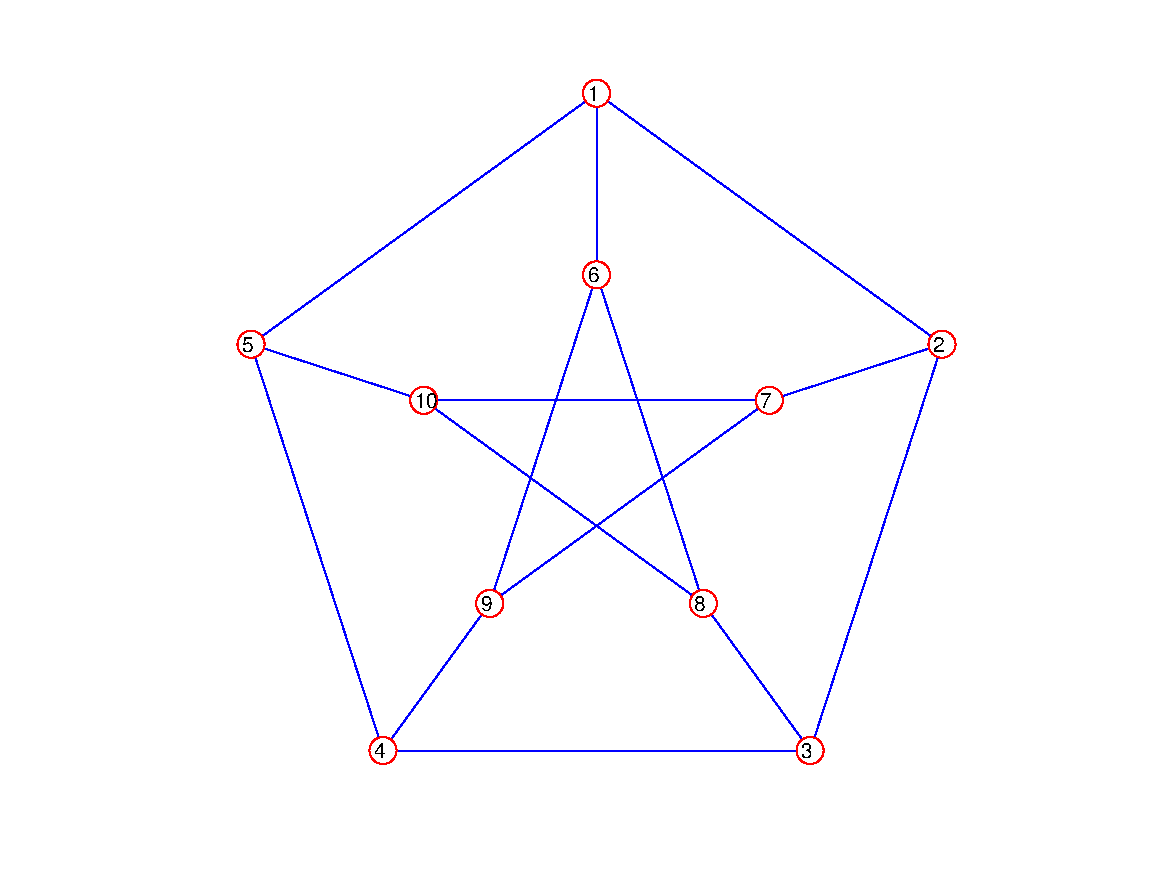
\includegraphics[scale=0.5]{figs/petersen}
  \end{center}
  \caption{Petersen's graph.}
  \label{fig:petersen}
\end{figure}
Note that the embedding of the graph is imparted to \verb|g| by the
command \verb|petersen|. In addition to \verb|ndraw|, \matgraph\ 
provides the following variations: \verb|draw| (draw the graph with
vertices drawn as hollow circles), \verb|ldraw| (draw the graph with
the vertices inscribed with their labels---different from their vertex
numbers), and \verb|cdraw| (draw the graph with colored vertices).
Type, for example, \verb|help cdraw| for more information.

It is well known that Petersen's graph is not Hamiltonian. To verify
this type:
\begin{verbatim}
>> hamiltonian_cycle(g)
ans =
     []
\end{verbatim}
The empty matrix indicates that no Hamiltonian cycle was
found. However, if we delete any vertex from \verb|g|, the graph is
Hamiltonian:
\begin{verbatim}
>> delete(g,1)
>> hamiltonian_cycle(g)
ans =
     1
     2
     3
     4
     9
     7
     5
     8
     6
\end{verbatim}
The command \verb|delete(g,1)| deletes vertex number 1 from the
graph. 

\textbf{Notice that the \texttt{delete} command changes the graph.} By a
bit of fancy footwork, \matgraph\ functions are able to modify
arguments of type \verb|graph|---this is counter to the usual \matlab\
call-by-value semantics. Many of the \matlab\ commands modify their
graph arguments, but the following convention is observed: If a
command is capable of modifying a graph, \emph{only the first argument
  to the command can by modified}.

\textbf{Notice that the vertices have been renumbered.} The output of
\verb|hamiltonian_cycle| reports that
$$
1 \to 2 \to 3 \to 4 \to 9 \to 7 \to 5 \to 8 \to 6 \to 1
$$ 
is a Hamiltonian cycle in \verb|g|. At first this may be confusing
since we had previous deleted vertex 1 from the graph. \matgraph\
follows the convention that the vertex set \emph{always} consists of
consecutive integers beginning with 1. When a vertex is deleted from a
graph, all vertices with higher numbers are renumbered accordingly. 
To see this, type this:
\begin{verbatim}
>> clf
>> ndraw(g)
\end{verbatim}
The result is shown in Figure~\ref{fig:petersen-vertex}.
\begin{figure}[ht]
  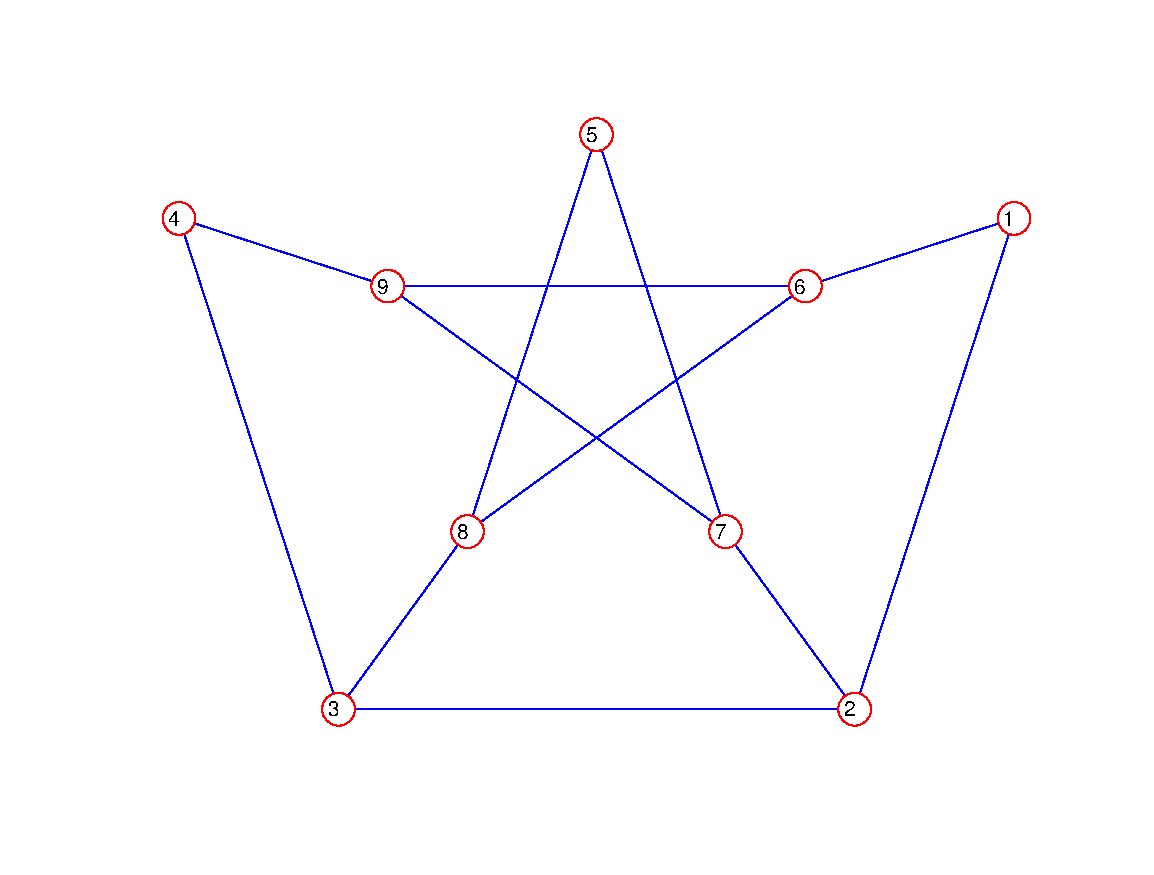
\includegraphics[scale=0.5]{figs/petersen-vertex}
  \caption{Petersen's graph with a vertex deleted is Hamiltonian.}
  \label{fig:petersen-vertex}
\end{figure}

Notice that we issued the \matlab\ command \verb|clf| before drawing
\verb|g|. The \verb|clf| command clears the current figure
window. This is necessary because \matgraph's drawing commands draw
their graphs on top of whatever is already in the figure window
(without erasing the figure window first). 

If we are done using the graph variable \verb|g|, we should \emph{not}
simply give the usual \matlab\ command \verb|clear g|. Rather, we do
this:
\begin{verbatim}
>> free(g)
>> clear g
\end{verbatim}
The command \verb|free(g)| releases the graph \verb|g|'s ``slot'' in a
hidden data structure. When \matgraph\ starts up (with the first
\verb|g=graph| command or by an explicit invocation of
\verb|graph_init|) a specific number of slots are allocated for graphs
(at this writing, 500 slots). Each time a graph variable is declared
(by typing \verb|g=graph|), one of these slots is used; the command
\verb|free(g)| releases the slot held by the graph. See the users'
guide for more detail. To wipe out the entire hidden data structure
(and all the graphs contained therein) you can use
\verb|graph_destroy|. 

One more important point. The typical behavior of \matlab's assignment
operator is to make a copy. So if \verb|A| is a matrix, \verb|B=A|
sets \verb|B| to be an independent copy of \verb|A|. Changes to
\verb|B| do not affect \verb|A|. However, \matgraph\ graph objects
behave differently. If \verb|g| is a graph, then the command
\verb|h=g| does \emph{not} make a separate copy of \verb|g|, and any
modification to \verb|h| also modifies \verb|g|. It is nearly certain
this is not the behavior you desire. Instead, do this:
\begin{verbatim}
>> g = graph
Graph with 0 vertices and 0 edges (full)
>> petersen(g)
>> h = graph
Graph with 0 vertices and 0 edges (full)
>> copy(h,g)
>> delete(h,1,2)
>> h
Graph with 10 vertices and 14 edges (full)
>> g
Graph with 10 vertices and 15 edges (full)
\end{verbatim}
The \verb|copy(h,g)| overwrites \verb|h| with an independent copy of
\verb|g|. 


\section{Basics}

\subsection{A path} One of the simplest graphs is a path on $n$
vertices, $P_n$. Here we create such a graph in \matgraph.
\begin{verbatim}
>> g = graph
Graph system initialized. Number of slots = 500.
Graph with 0 vertices and 0 edges (full)
>> for k=1:9, add(g,k,k+1), end
>> ndraw(g)
\end{verbatim}
This creates the graph $P_{10}$ and draws it in a figure window.
Notice that the command \verb|add(g,u,v)| adds the edge $uv$ to the
graph. The variables $u$ and $v$ must be distinct positive integers;
otherwise the command has no effect. If vertices $u$ and $v$ are
already in the graph, the edge $uv$ is simply added. However, if a
graph has $n$ vertices and either $u$ or $v$ is greater than $n$, then
the graph's vertex set is first expanded to $\max\{u,v\}$ vertices and
then the edge is added. [Remember, the vertex set of a graph in
\matgraph\ is \emph{always} of the form $\{1,2,\ldots,n\}$.]

Notice that the drawing of \verb|g| places the vertices around a
circle. If a graph does not have an embedding (e.g., the
\verb|petersen| command imparts an embedding to its argument), then
then the drawing commands (such as \verb|ndraw|) give the graph a
default embedding by placing the vertices around a circle. 

Now here is a simpler way to create (and view) $P_{10}$:
\begin{verbatim}
>> path(g,10)
>> clf
>> ndraw(g)
\end{verbatim}
The command \verb|path(g,10)| overwrites \verb|g| with a path on 10
vertices together with a sensible embedding---the vertices are
arranged in a straight line. 

\subsection{Adding and deleting} 
Let's create the graph formed by deleting a perfect matching from
$K_{10}$. Here are the commands:
\begin{verbatim}
>> complete(g,10)
>> for k=1:5, delete(g,k,k+5), end
>> clf
>> ndraw(g)
\end{verbatim}
The command \verb|complete(g,10)| overwrites \verb|g| with $K_{10}$. (We
assume that we are simply continuing from the previous section so the
graph \verb|g| has already been declared.) The \verb|delete(g,u,v)|
command deletes the edge $uv$ from the graph (assuming it exists).
This 3-argument version of \verb|delete| does not remove any vertices
from the graph.

To delete vertex $u$ from a graph (and all its incident edges)
give the command \verb|delete(g,u)|. Type \verb|help graph/delete| to
see all the various ways \verb|delete| can remove vertices and edges
from a graph. 

To delete all vertices (and hence, all edges) from a graph, type
\verb|resize(g,0)|. To delete all edges (but no vertices) from a
graph, type \verb|clear_edges(g)|. 

\medbreak 

Creating the graph formed from $K_{5,5}$ by deleting a perfect
matching is similar:
\begin{verbatim}
>> complete(g,5,5)
>> for k=1:5, delete(g,k,k+5), end
>> clf
>> ndraw(g)
\end{verbatim}
The command \verb|complete(g,m,n)| overwrites \verb|g| with the
complete bipartite graph $K_{m,n}$. Type \verb|help graph/complete| to
see what else \verb|complete| can do.

\medbreak

Now try this:
\begin{verbatim}
>> resize(g,0)
>> add(g,3,6)
>> clf
>> ndraw(g)
\end{verbatim}
The command \verb|resize(g,0)| converts \verb|g| to an empty
(vertexless) graph. \verb|add(g,3,6)| asks to add an edge between
vertices 3 and 6, but since these vertices are not (yet) in the graph,
the vertex set of \verb|g| is expanded to $\{1,2,3,4,5,6\}$ and then
the edge is added. Consequently, there are four isolated vertices in
\verb|g| as the picture reveals.

\medbreak
Next we create the M\"obius ladder on 12 vertices (a 12-cycle
plus edges between diametrically opposite vertices). 
\begin{verbatim}
>> cycle(g,12)
>> elist = [1:6;7:12]'
elist =
     1     7
     2     8
     3     9
     4    10
     5    11
     6    12
>> add(g,elist)
>> clf; ndraw(g)
\end{verbatim}
\verb|cycle(g,12)| overwrites \verb|g| with $C_{12}$. Next, we prepare
a $6\times2$ matrix \verb|elist| that specifies the extra edges we
plan to add to \verb|g|. The line \verb|elist = [1:6;7:12]'| is
standard \matlab\ to create this matrix. Then \verb|add(g,elist)| adds
all the edges in \verb|elist| to \verb|g|.


\subsection{Neighbors, degrees, etc.}

Create a grid graph like this:
\begin{verbatim}
>> grid(g,3,4)
>> clf;ndraw(g)
>> nv(g)
ans =
    12
>> ne(g)
ans =
    17
\end{verbatim}
The grid is drawn nicely as shown in Figure~\ref{fig:grid34}.
\begin{figure}[ht]
  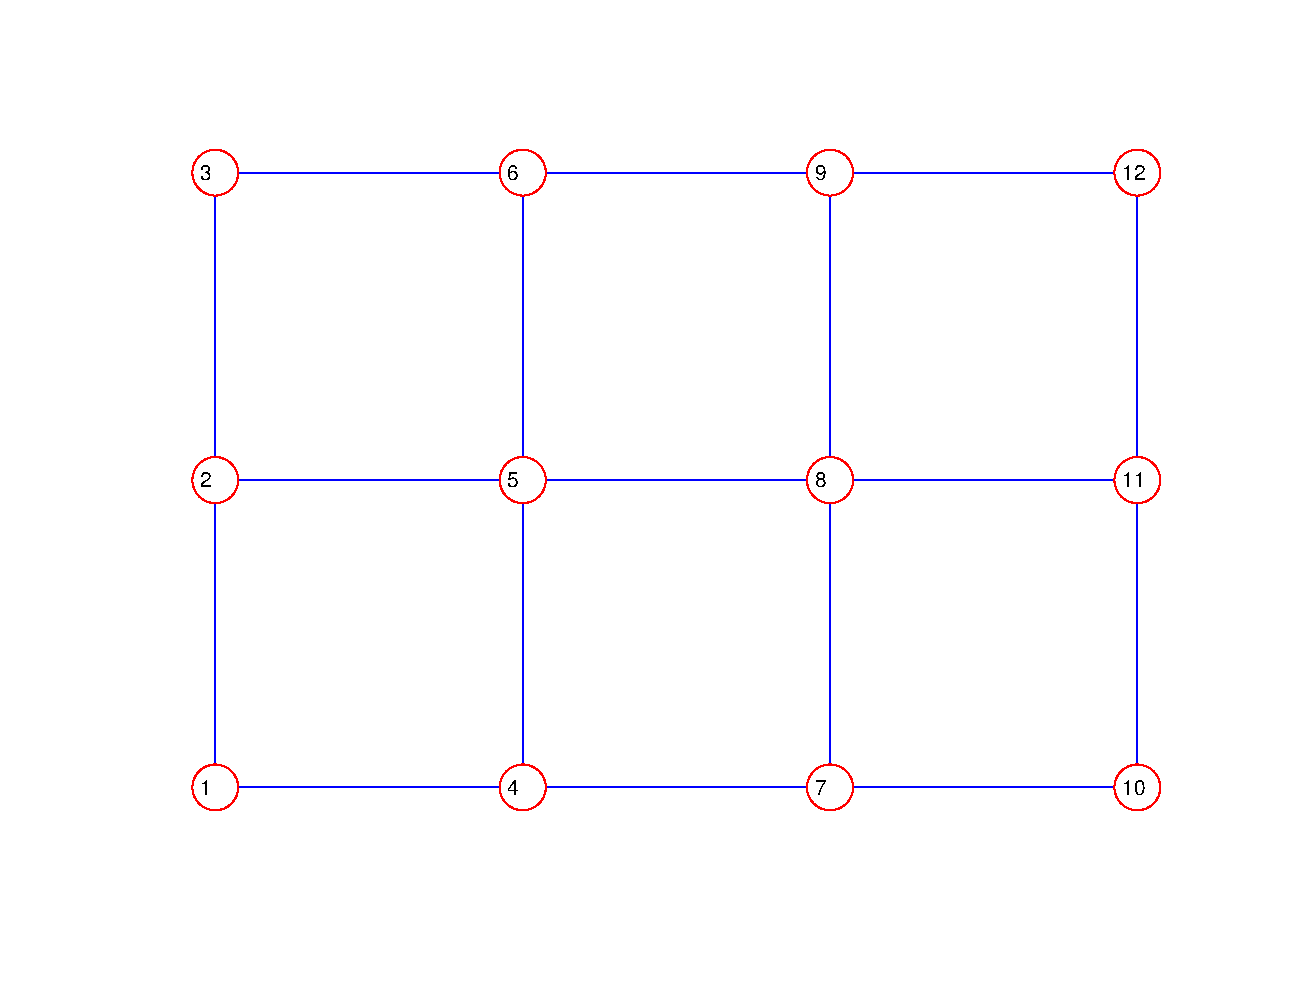
\includegraphics[scale=0.5]{figs/grid34}
  \caption{The $3\times4$ grid graph.}
  \label{fig:grid34}
\end{figure}
Notice that \verb|nv| and \verb|ne| report the number of vertices and
edges, respectively, of the graph. Also try \verb|size(g)|,
\verb|disp(g)|, or simply typing \verb|g| on a line by itself.

We can learn the degree of a vertex, or the entire degree sequence of
the graph, like this:
\begin{verbatim}
>> deg(g,1)
ans =
     2
>> deg(g,2)
ans =
     3
>> deg(g)
ans =
     2    3    2    3    4    3    3    4    3    2    3    2
\end{verbatim}
To learn the neighbors of a vertex, we have two choices:
\begin{verbatim}
>> neighbors(g,2)
ans =
     1     3     5
>> g(2)
ans =
     1     3     5
\end{verbatim}
[Note, the syntax \verb|g(v)| does not seem to work inside \verb|.m|
file functions.]

To test if two vertices are adjacent we can use the \verb|has| command
or the syntax \verb|g(u,v)| [which does not seem to work inside
\verb|.m| file functions]. 
\begin{verbatim}
>> has(g,1,2)
ans =
     1
>> has(g,1,5)
ans =
     0
>> g(1,2)
ans =
     1
>> g(1,5)
ans =
     0
\end{verbatim}

We can verify that this graph is connected
\begin{verbatim}
>> isconnected(g)
ans =
     1
\end{verbatim}
and find a shortest path between vertices 1 and 12:
\begin{verbatim}
>> find_path(g,1,12)
ans =
     1     2     3     6     9    12
\end{verbatim}
Try \verb|dist(g,1,12)| to see that the distance between these
vertices is 5.


\subsection{Matrices}

To get the adjacency matrix of, say, the Petersen graph, do this:
\begin{verbatim}
>> petersen(g)
>> A = matrix(g)
A =
     0     1     0     0     1     1     0     0     0     0
     1     0     1     0     0     0     1     0     0     0
     0     1     0     1     0     0     0     1     0     0
     0     0     1     0     1     0     0     0     1     0
     1     0     0     1     0     0     0     0     0     1
     1     0     0     0     0     0     0     1     1     0
     0     1     0     0     0     0     0     0     1     1
     0     0     1     0     0     1     0     0     0     1
     0     0     0     1     0     1     1     0     0     0
     0     0     0     0     1     0     1     1     0     0
\end{verbatim}
Next, we attempt to find the eigenvalues of this matrix, but run into
trouble:
\begin{verbatim}
>> eig(A)
??? Function 'eig' is not defined for values of class 'logical'.
\end{verbatim}
The problem is that \matgraph's \verb|matrix| command returns a
Boolean matrix (entries represent \texttt{true} and \texttt{false}),
but it is simple to convert this to a numerical matrix and get the
eigenvalues:
\begin{verbatim}
>> A = double(A);
>> eig(A)
ans =
   -2.0000
   -2.0000
   -2.0000
   -2.0000
    1.0000
    1.0000
    1.0000
    1.0000
    1.0000
    3.0000
\end{verbatim}
Use \verb|laplacian| to get the Laplacian matrix of a graph. 

The command \verb|spy(g)| is equivalent to \verb|spy(matrix(g))|; this
creates a square image with a dot in position $i,j$ exactly when $ij$
is an edge of $g$. 

It is also possible to define a graph by specifying its adjacency
matrix:
\begin{verbatim}
>> A = ones(6)-eye(6)
A =
     0     1     1     1     1     1
     1     0     1     1     1     1
     1     1     0     1     1     1
     1     1     1     0     1     1
     1     1     1     1     0     1
     1     1     1     1     1     0
>> set_matrix(g,A)
>> g
Graph with 6 vertices and 15 edges (full)
\end{verbatim}

See also: \verb|incidence_matrix|.


\subsection{Standard graph constructors}

\matgraph\ includes many functions for creating specific, standard
graphs. We have encountered a few already: \verb|path|, \verb|cycle|,
\verb|complete|, \verb|petersen|, and \verb|grid|. 

In addition to these, there are built-in methods for creating the
Platonic solid graphs (for example, \verb|dodecahdron|), wheels, Paley
graphs, and so forth. See the on-line documentation (in the
\verb|matgraph/html| directory) for a complete list of all graph
methods.

Graphs can also be built up from other graphs using graph operations;
these are explored in \S\ref{sect:ops}.

Worthy of special mention are various methods to generate random
graphs including \verb|random|, \verb|random_bipartite|,
\verb|random_regular|, and \verb|random_tree|.


\section{Embeddings}

\subsection{Basics}

As we have seen, graphs created in \verb|matgraph| can be drawn on the
screen. A graph may have an embedding that is simply a specification
of $x,y$-coordinates for all of the vertices. Edges are always drawn
as line segments.

Some graph constructors (e.g., \verb|petersen|) imbue their graphs
with a prespecified embedding. However, if we start with a new graph
and simply add vertices and edges, no embedding is created for the
graph:
\begin{verbatim}
>> g = graph
Graph system initialized. Number of slots = 500.
Graph with 0 vertices and 0 edges (full)
>> for k=1:5, add(g,k,k+1), end
>> g
Graph with 6 vertices and 5 edges (full)
>> hasxy(g)
ans =
     0
\end{verbatim}
This creates the path $P_6$ but no embedding is associated with the
graph; this is observed with the \verb|hasxy| command. 

If we try to draw a graph that lacks an embedding, \matgraph\ gives
the graph a default embedding in which the vertices are placed around
a circle. 
\begin{verbatim}
>> draw(g)
>> hasxy(g)
ans =
     1
\end{verbatim}
We can specify the embedding for a graph by giving specific
$x,y$-coordinates. Suppose we want to site the vertices of $P_6$ at
$(1,0)$, $(2,0)$, \ldots, $(6,0)$; we can do this:
\begin{verbatim}
>> xy = [ 1:6 ; zeros(1,6) ]'
xy =
     1     0
     2     0
     3     0
     4     0
     5     0
     6     0
>> embed(g,xy)
>> clf;draw(g)
\end{verbatim}

If a graph possesses an embedding, \verb|rmxy(g)| removes the
embedding. To see the embedding of a graph, use \verb|getxy|.

A random embedding can be given to a graph with \verb|randxy(g)|. See
also the \verb|scale| function.


\subsection{Automatic graph layout}

\matgraph's default embedding---vertices uniformly around a
circle---is usually unaesthetic and difficult to read. Fortunately,
\matgraph\ provides a way to create embeddings automatically.
Unfortunately, the one viable method we provide---\verb|distxy|---is
slow and requires\footnote{If the Optimization Toolbox is not included
  with your version of \matlab, it is available (for a fee) from The
  MathWorks.}  the Optimization Toolbox. Nevertheless, \verb|distxy|
gives reasonable results for moderately sized graphs. We invite
readers who are expert in graph drawing algorithms to submit
alternatives for inclusion in future releases of \matgraph.

The \verb|distxy| embedding attempts to place vertices in a graph in
the plane so that their graph theoretic distance equals the embedded
vertices Euclidean distance. This is possible for path graphs, but
otherwise is unattainable. Instead, we create a score function that
measures how closely we achieve this goal and then use the services of
the Optimization Toolbox to find a (local) minimum solution. Here is
an example.
\begin{verbatim}
>> resize(g,0)
>> random_tree(g,10)
>> clf;draw(g)
\end{verbatim}
This creates a random tree with $10$ vertices and displays the tree in
its default embedding. See the left portion of Figure~\ref{fig:randtree}.
\begin{figure}[ht]
  \begin{center}
    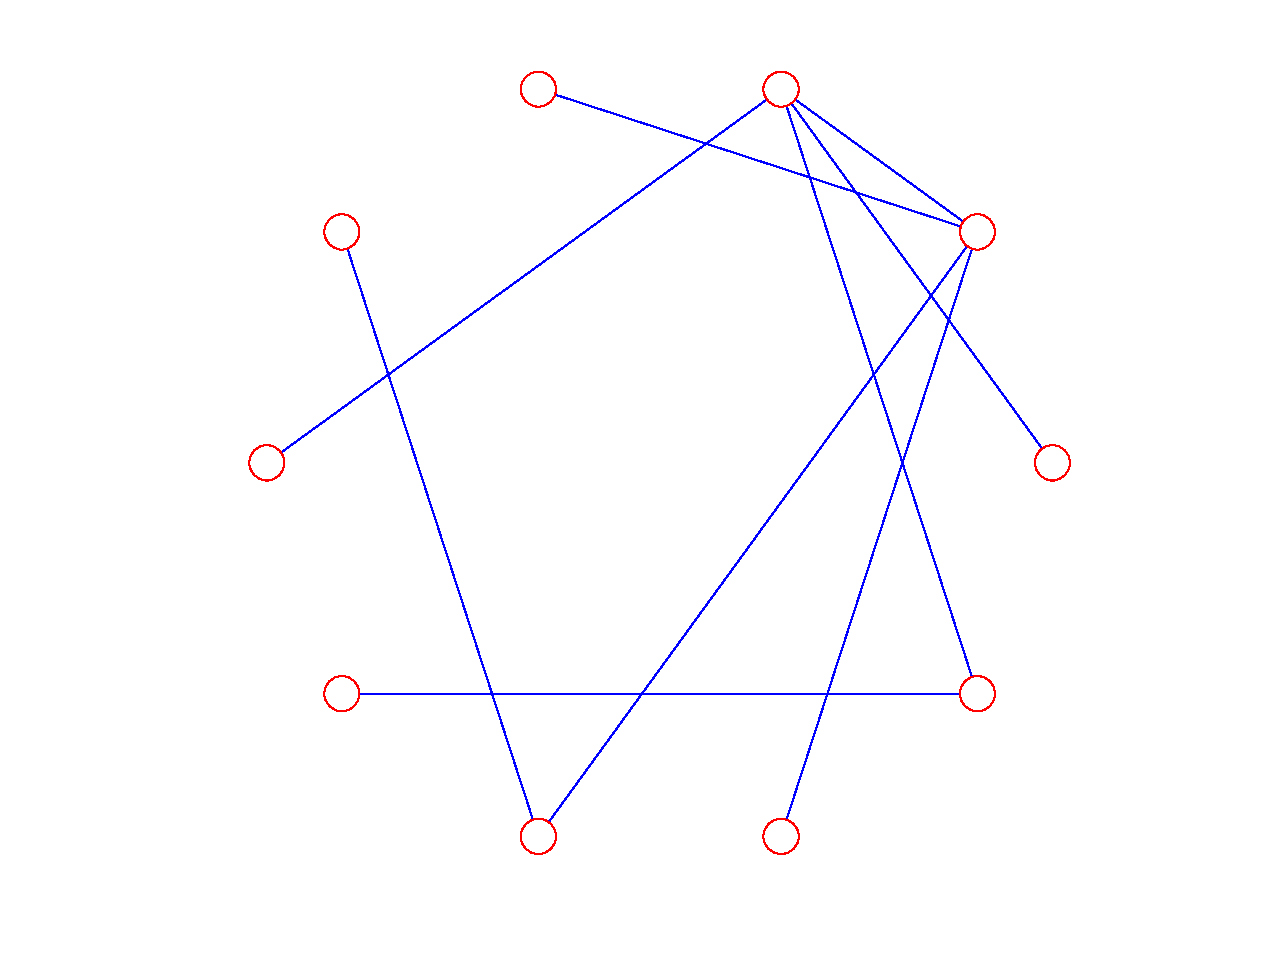
\includegraphics[scale=0.3]{figs/randtree-yuck}
    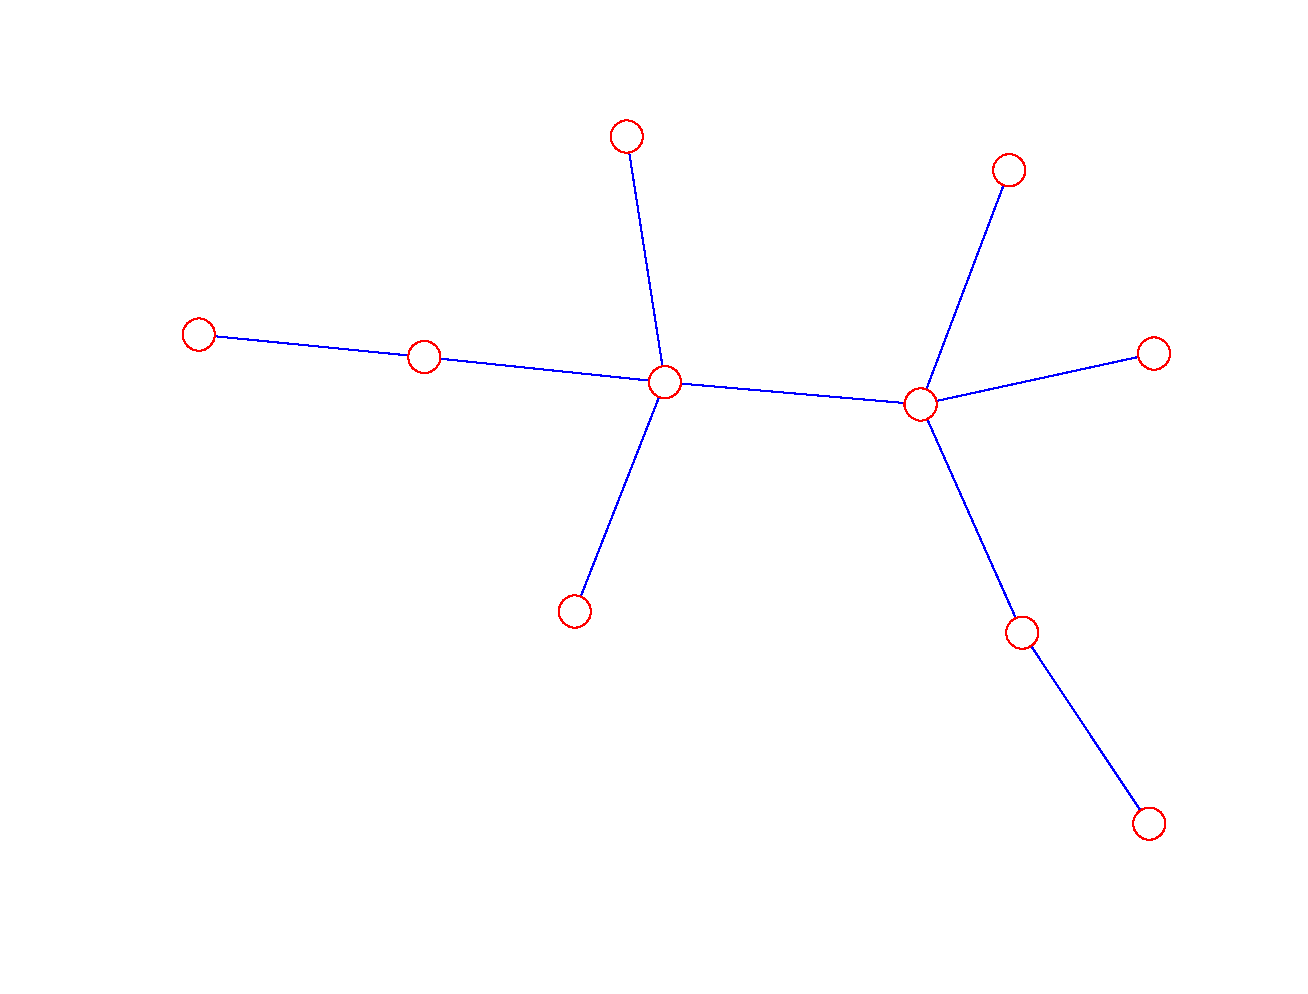
\includegraphics[scale=0.3]{figs/randtree-nice}
  \end{center}
  \caption{A random tree with its default embedding (left)
    and with a nice embedding found by \texttt{distxy} (right).}
  \label{fig:randtree}
\end{figure}
Now we compute an embedding using \verb|distxy|.
\begin{verbatim}
>> distxy(g)
Optimization terminated: relative function value
 changing by less than OPTIONS.TolFun.
Embedding score = 2.7511
Elapsed time is 0.941816 seconds.
ans =
    2.7511
>> clf;draw(g)
\end{verbatim}
The result is show in the right portion of Figure~\ref{fig:randtree}.

\section{Helper Classes: Partitions and Permutations}

\matgraph\ includes two classes that are useful for supporting work:
partitions and permutations.

\subsection{Partitions}
A \emph{partition} is a set of pairwise disjoint, nonempty subsets of
a set $A$ whose union is $A$. In \matgraph, all partitions must be of
a set of the form $[n]=\{1,2,\ldots,n\}$. \verb|partition| variables
do not need to be declared (only \verb|graph| objects require that
special treatment).

Partitions are useful in graph theory. In \matgraph\, the functions to
find the connected components of a graph or to find a coloring of a
graph return \verb|partition| objects.

There are a few ways to create a partition. The most basic is this:
\begin{verbatim}
>> p = partition(8)
{ {1} {2} {3} {4} {5} {6} {7} {8} }
\end{verbatim}
The command \verb|partition(n)| creates a default partition of $[n]$
in which each element is in a part by itself. 

Alternatively, we can form a \verb|partition| from a \matlab\ cell
array. Each cell in the cell array is a list (vector) of integers;
taken together, these cells should contain all of the numbers from $1$
to $n$ (for some $n$) exactly once. Here is an example.
\begin{verbatim}
>> c = cell(3,1);
>> c{1} = [1 3 5];
>> c{2} = [4 6 7];
>> c{3} = [2 8];
>> p = partition(c)
{ {1,3,5} {2,8} {4,6,7} }
\end{verbatim}
The statement \verb|c = cell(3,1);| builds a $3\times1$ cell array
(a fundamental \matlab\ data structure). The next three lines populate
the array with three lists of numbers. Finally, the statement
\verb|p = partition(c)| assigns to \verb|p| a partition with the
expected blocks. 

The \verb|merge| command is used to combine parts in a
partition. Continuing with the example above, we type this:
\begin{verbatim}
>> merge(p,1,2)
{ {1,2,3,5,8} {4,6,7} }
>> p
{ {1,3,5} {2,8} {4,6,7} }
\end{verbatim}
\verb|merge(p,1,2)| forms a new partition in which the parts
containing elements 1 and 2 are combined into a single part. Note that
\verb|merge| does not alter \verb|p|; this is normal \matlab\
behavior. 


Now try this:
\begin{verbatim}
>> p(1)
ans =
     1     3     5
>> p(1,2)
ans =
     0
\end{verbatim}
The command \verb|p(v)| returns (as a list) the elements in \verb|v|'s
block. The command \verb|p(v,w)| returns 1 (true) if \verb|v| and
\verb|w| are in the same block, and returns 0 (false) otherwise. 

There are other ways to extract the parts of a partition. 
\begin{verbatim}
>> pts = parts(p);
>> pts{1}
ans =
     1     3     5
>> pts{2}
ans =
     2     8
>> pts{3}
ans =
     4     6     7
\end{verbatim}
The function \verb|parts| returns the parts of a partition as a cell
array.
\begin{verbatim}
>> array(p)
ans =
     1     2     1     3     1     3     3     2
\end{verbatim}
The \verb|array| function returns an index number for each element; an
element has index number $i$ if it is in the $i^{\text{th}}$ part of
the partition.

The binary operators \verb|==| and \verb|!=| can be used to test if
two partitions are equal or unequal. 

The binary operators \verb|+| and \verb|*| can be used to compute the
join and meet of two partitions. 

\verb|nv(p)| returns the size of the ground set of the partition and
\verb|np(p)| returns the number of blocks in the partition. See also
\verb|size(p)|. 


\subsection{Permutations}

A \emph{permutation} is a bijection of a set $A$ to itself. In
\matgraph, the set $A$ is always of the form $[n] = \{1,2,\ldots,
n\}$.

A new permutation is created with the \verb|permutation| function:
\begin{verbatim}
>> permutation(9)
(1)(2)(3)(4)(5)(6)(7)(8)(9)
\end{verbatim}
The \verb|permutation(n)| command creates the identity permutation of
$[n]$. 

The \verb|permutation| function can also be used to create a
permutation from a list of numbers. 
\begin{verbatim}
>> vec = [ 1 3 5 2 4 6 ];
>> permutation(vec)
(1)(2,3,5,4)(6)
>> 
\end{verbatim}
Here, the permutation is given by the matrix
$$
\pi = 
\begin{bmatrix}
  1&2&3&4&5&6 \\
  1&3&5&2&4&6
\end{bmatrix}
$$
The list \verb|vec| gives the bottom row. This notation means that
$\pi(1)=1$, $\pi(2)=3$, $\pi(3)=5$, $\pi(4)=2$, $\pi(5)=4$, and
$\pi(6)=6$. 

A random permutation can be created like this:
\begin{verbatim}
>> p = permutation(9);
>> p = random(p)
(1,7,6,2,4,9)(3,8)(5)
\end{verbatim}

\matgraph\ defines \verb|*| to denote permutation composition. The
notation \verb|p(j)| applies the permutation \verb|p| to element
\verb|j|:
\begin{verbatim}
>> p(2)
ans =
     4
\end{verbatim}

The inverse of a permutation can be calculated like this:
\begin{verbatim}
>> inv(p)
(1,9,4,2,6,7)(3,8)(5)
>> p^-1
(1,9,4,2,6,7)(3,8)(5)
\end{verbatim}
In general, \verb|p^m| is the $m$-fold composition of \verb|p| with
itself; \verb|m| may be negative.

\begin{verbatim}
>> matrix(p)
ans =
     0     0     0     0     0     0     0     0     1
     0     0     0     0     0     1     0     0     0
     0     0     0     0     0     0     0     1     0
     0     1     0     0     0     0     0     0     0
     0     0     0     0     1     0     0     0     0
     0     0     0     0     0     0     1     0     0
     1     0     0     0     0     0     0     0     0
     0     0     1     0     0     0     0     0     0
     0     0     0     1     0     0     0     0     0
>> array(p)
ans =
     7     4     8     9     5     2     6     3     1
\end{verbatim}
\verb|matrix(p)| creates a permutation matrix and \verb|array(p)|
gives the lower row of the permutation when written in $2\times
n$-matrix notation. 

\begin{verbatim}
>> c = cycles(p);
>> c{1}
ans =
     1     7     6     2     4     9
>> c{2}
ans =
     3     8
>> c{3}
ans =
     5
\end{verbatim}
The \verb|cycles| function creates a cell array containing the
permutation's cycles. 


\section{Vertex Numbers and Labels}

\matgraph\ rigidly enforces the rule that the vertex set of any graph
must be of the form $\{1,2,\ldots,n\}$. If we delete some vertices of
the graph, other vertices are renumbered and this can make associating
a vertex's original number with its new number difficult. Also, one
may wish to give a vertex an alphanumeric name. 

To deal with these issues, \matgraph\ provides a mechanism for
labeling the vertices of a graph with arbitrary text strings. 

Try this:
\begin{verbatim}
>> g = graph
Graph with 0 vertices and 0 edges (full)
>> cycle(g,8)
>> label(g)
>> label(g,3,'X')
>> delete(g,4)
>> ldraw(g)
\end{verbatim}
When a graph is first created, there are no labels associated with its
vertices. The command \verb|label(g)| causes \verb|g|'s vertices to be
given default labels. The default label assigned to a vertex is simply
a string containing the digits of its vertex number (e.g., vertex 23
would be labeled \verb|'23'|). 

The command \verb|label(g,3,'X')| labels vertex number 3 with the
string \verb|'X'|. The label need not be a single character, we could
have labeled this vertex like this: \verb|label(g,3,'three')|. 

Next we delete vertex number 4. This renumbers vertices 5 through 8 to
new numbers 4 through 7. However, the label associated with a vertex
remains the same. That is, the vertex now numbered 4 (and formally
numbered 5) has the label \verb|'5'|. 

Finally, the \verb|ldraw| command draws the graph with each vertex's
label written in the middle of its circle. See
Figure~\ref{fig:labeled-path}. 
\begin{figure}[ht]
  \begin{center}
    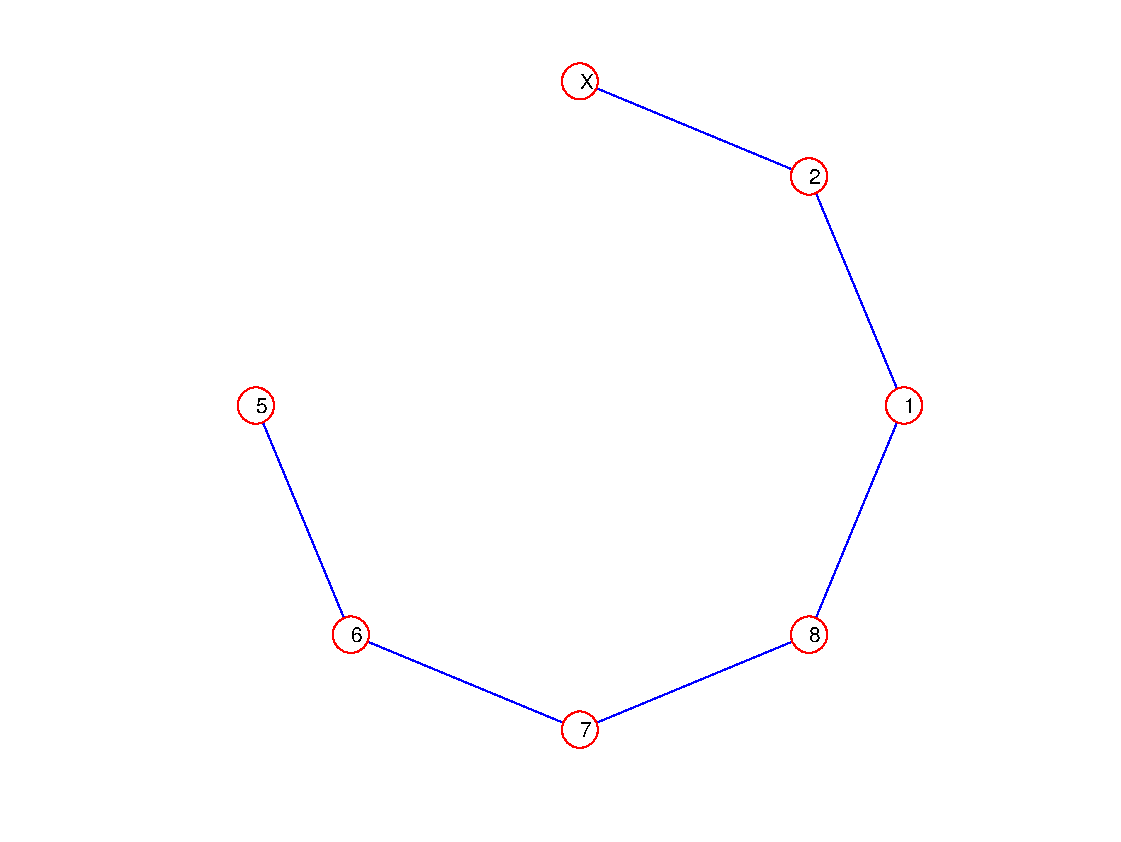
\includegraphics[scale=0.5]{figs/labeled-path}
  \end{center}
  \caption{A drawing of a labeled graph.}
  \label{fig:labeled-path}
\end{figure}

To learn the label of a vertex, or to extract a cell array containing
all the labels of a graph, use \verb|get_label|. 

It is possible to assign two different vertices the same label, so
there need not be a one-to-one correspondence between vertices and
label. 


\section{Graph Operations}
\label{sect:ops}

\matgraph\ provides various operations to perform on graphs. Here we
present some examples.
\begin{verbatim}
>> g = graph
Graph system initialized. Number of slots = 500.
Graph with 0 vertices and 0 edges (full)
>> complete(g,[2,3,4])
>> deg(g)
ans =
     7     7     6     6     6     5     5     5     5
>> complement(g)
>> deg(g)
ans =
     1     1     2     2     2     3     3     3     3
>> 
\end{verbatim}
This sets \verb|g| to be the complete multipartite graph $K_{2,3,4}$,
and then overwrites \verb|g| with its own complement,
$\overline{K_{2,3,4}}$. This is equivalent to the disjoint union
$K_2\oplus K_3 \oplus K_4$. \matgraph\ can compute disjoint unions of
graphs like this:
\begin{verbatim}
>> cycle(g,5)
>> h = graph;
>> cycle(h,6)
>> k = graph;
>> disjoint_union(k,g,h)
>> k
Graph with 11 vertices and 11 edges (full)
\end{verbatim}
This code resets \verb|g| to be the 5-cycle, defines a new graph
variable \verb|h| to be a 6-cycle, and then places the disjoint union
of these graphs in a third graph \verb|k|. See also the \verb|union|
command. 

The complement of $C_5 \oplus C_6$ can now be computed using
\verb|complement(k)|. Alternatively, we can do this:
\begin{verbatim}
>> complement(g);   % g is now the complement of C_5 (which is C_5)
>> complement(h);   % h is now the complement of C_6
>> join(k,g,h)
>> h
Graph with 6 vertices and 9 edges (full)
\end{verbatim}
The \verb|join| commands overwrites its first argument with a graph
formed from the disjoint union of its second and third arguments, plus
all possible edges between these latter two graphs. 

The \emph{Cartesian product} of graphs $G$ and $H$ is a new graph
$G\times H$ defined as follows:
\begin{align*}
  V(G\times H) &= V(G) \times V(H) = \{(v,w): v \in V(G), w \in V(H)\}
  \\
  E(G\times H) &= \bigl\{ \{(v_1,w_1),(v_2,w_2)\} :
  [v_1v_2 \in E(G) \text{ and } w_1=w_2] \text{ or }
  [v_1=v_2 \text{ and } w_1w_2 \in E(H)] \bigr\}
\end{align*}
We illustrate how to calculate Cartesian product in \matgraph:
\begin{verbatim}
>> clf;draw(k)
>> cycle(g,10)
>> cycle(h,3)
>> cartesian(k,g,h)
>> k
Graph with 30 vertices and 60 edges (full)
>> distxy(k)
Optimization terminated: relative function value
 changing by less than OPTIONS.TolFun.
Embedding score = 51.6601
Elapsed time is 5.263166 seconds.
ans =
   51.6601
>> clf;draw(k)
\end{verbatim}
The resulting drawing is shown in Figure~\ref{fig:product-graph}.
\begin{figure}[ht]
  \begin{center}
    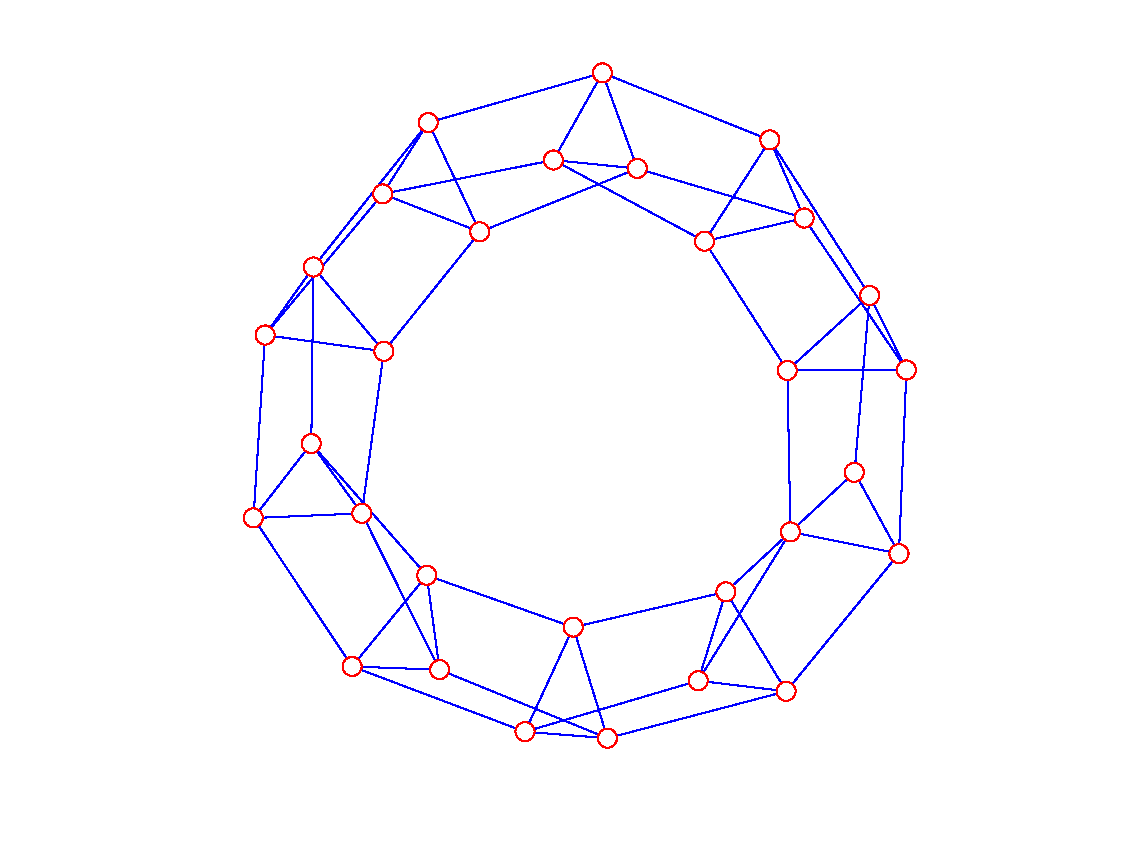
\includegraphics[scale=0.5]{figs/product-graph}
  \end{center}
  \caption{The Cartesian product $C_{10}\times C_3$.}
  \label{fig:product-graph}
\end{figure}
The hypercube $Q_n$ is defined to be the $n$-fold product $K_2 \times
K_2 \times \cdots \times K_2$. The command \verb|cube(g,n)| overwrites
\verb|g| with the graph $Q_n$. 

\matgraph\ can find spanning trees in (connected) graphs. The two
commands \verb|bfstree| and \verb|dfstree| find breadth-first and
depth-first spanning trees of their respective graphs. 
\begin{verbatim}
>> dodecahedron(g)
>> bfstree(h,g)
>> clf; draw(g,':')
>> draw(h)
\end{verbatim}
The command \verb|bfstree(h,g)| overwrites \verb|h| with a
breadth-first spanning tree of \verb|g| rooted at vertex 1. (To start
from another vertex, use \verb|bfstree(h,g,v)|.) We then draw the
original graph \verb|g| using dotted lines (the extra argument to
\verb|draw|) and then draw the spanning tree (using the default solid
lines) without erasing the first drawing. The result is in
Figure~\ref{fig:bfstree}.
\begin{figure}[ht]
  \begin{center}
    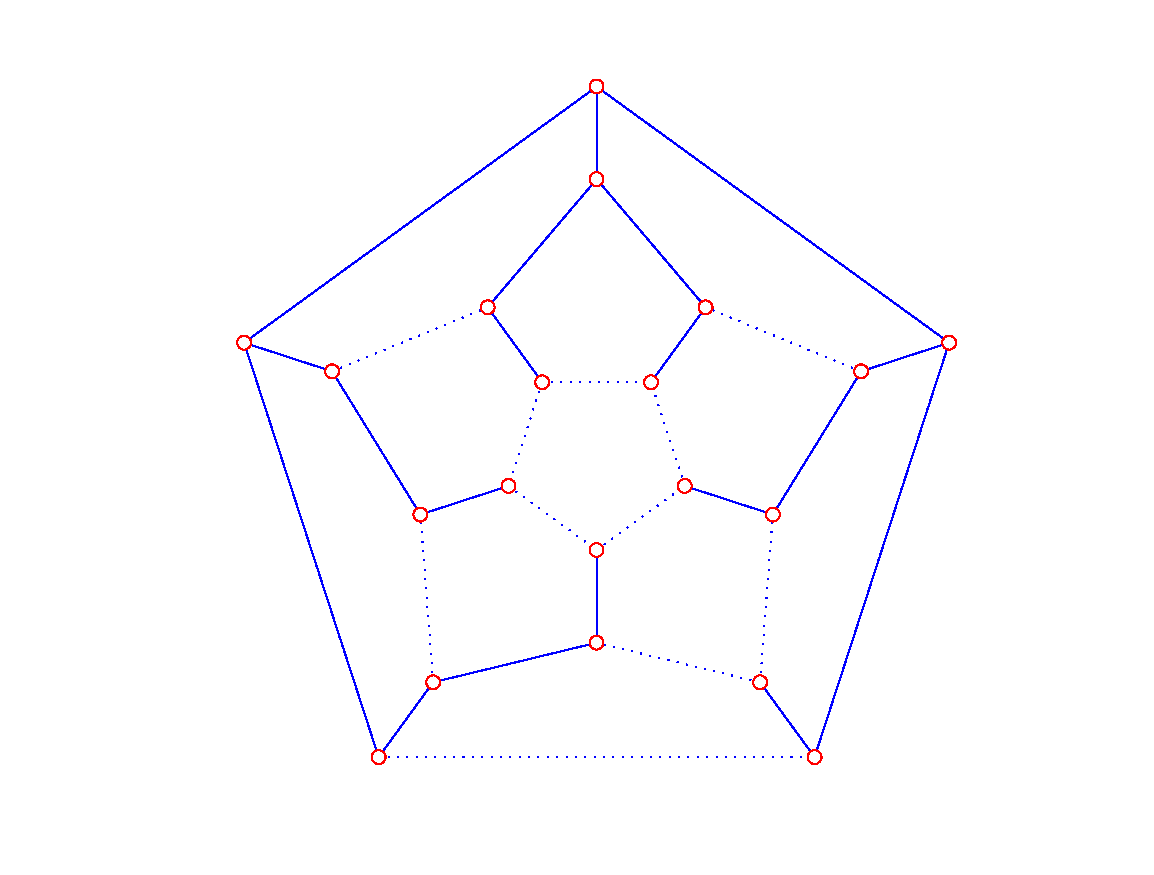
\includegraphics[scale=0.5]{figs/bfstree}
  \end{center}
  \caption{A breadth-first spanning tree of the dodecahedron graph.}
  \label{fig:bfstree}
\end{figure}

\matgraph\ can also find Hamiltonian cycles (but only in small
graphs). Here's an example.
\begin{verbatim}
>> dodecahedron(g)
>> hamiltonian_cycle(h,g);
>> clf;draw(g,':')
>> draw(h)
\end{verbatim}
The result is in Figure~\ref{fig:ham-cycle}.
\begin{figure}[ht]
  \begin{center}
    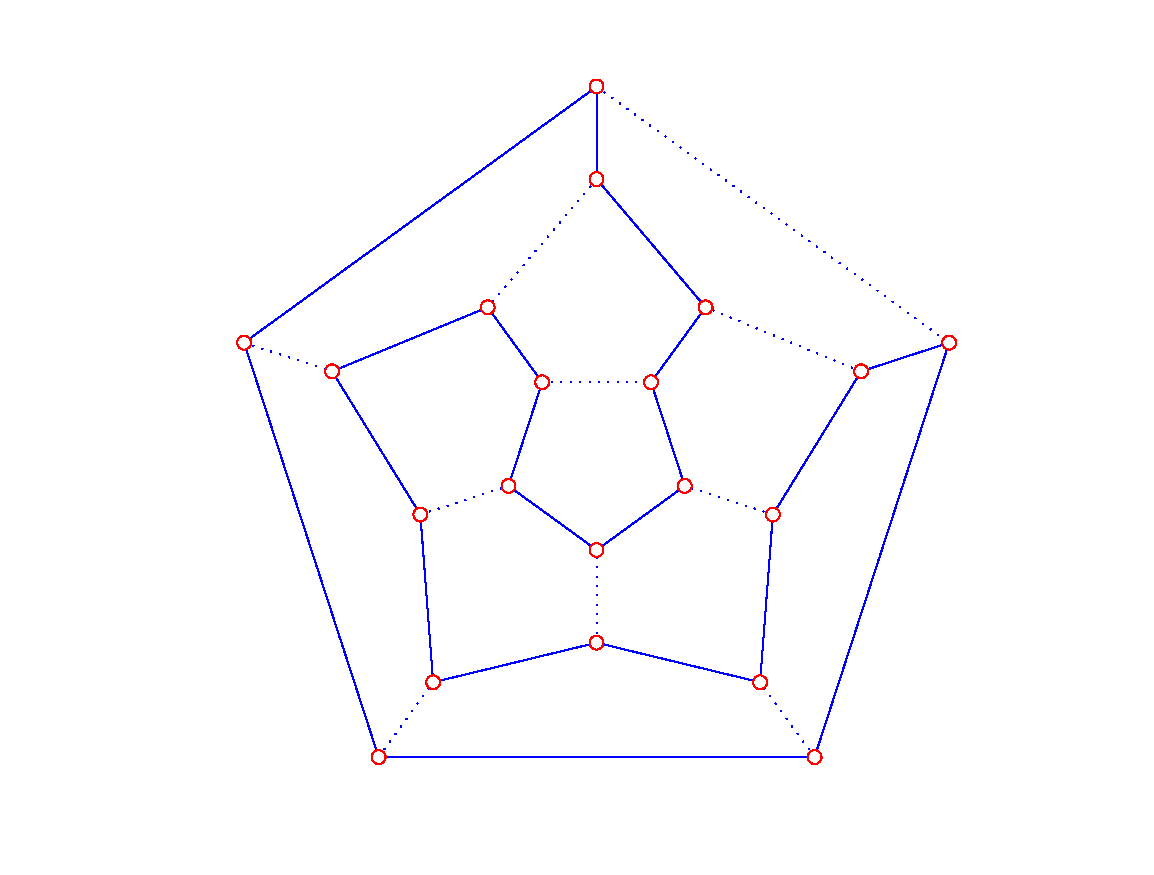
\includegraphics[scale=0.5]{figs/ham-cycle}
  \end{center}
  \caption{A Hamiltonian cycle in the dodecahedron graph.}
  \label{fig:ham-cycle}
\end{figure}

\matgraph\ can form induced subgraphs.
\begin{verbatim}
>> cycle(g,10)
>> induce(h,g,[1 2 3 4 5 9])
>> h
Graph with 6 vertices and 4 edges (full)
\end{verbatim}
The \verb|induce| command above overwrites \verb|h| with the induced
subgraph of \verb|g| generated by the vertex set
$\{1,2,3,4,5,9\}$. This makes \verb|h| the graph consisting of a
5-path (on vertices 1 through 5) plus an isolated vertex (now numbered
6 in \verb|h|). The new vertex 6 in \verb|h| inherits the label of
vertex 9 in \verb|g| (assuming \verb|g| was labeled).

The \verb|trim| command is useful for removing vertices of degree
0. More generally, \verb|trim(g,d)| removes all vertices of degree at
most $d$ from \verb|g|, and then repeats this operation on the
resulting graph until \verb|g| has minimum degree at least $d+1$ (or
all vertices have been deleted).



\section{Graph Computations}

\subsection{Basic invariants}
As discussed earlier, \verb|nv(g)| and \verb|ne(g)| returns the number
of vertices and edges in \verb|g|, respectively. \verb|size(g)|
reports the same information as a list. 

The independence number, clique, and domination number can be computed
by \matgraph; note that the computation of these invariants requires
\matlab's Optimization Toolbox.
\begin{verbatim}
>> g = graph
Graph system initialized. Number of slots = 500.
Graph with 0 vertices and 0 edges (full)
>> icosahedron(g)
>> alpha(g)  % compute the independence number
Optimization terminated.
ans =
     3
>> omega(g)  % compute the clique number
Optimization terminated.
ans =
     3
>> dom(g)    % compute the domination number
Optimization terminated.
ans =
     2
\end{verbatim}
In each case, we can find the realizing set (independent, clique, or
dominating) with an extra output argument:
\begin{verbatim}
>> [d,S] = dom(g)
Optimization terminated.
d =
     2
S =
     4
     7
>> sort([g(4),g(7),4,7])
ans =
    1    2    3    4    5    6    7    8    9   10   11   12
\end{verbatim}

\subsection{Connection}
\matgraph\ can determine if a graph is connected, find paths between
vertices, and determine distances. We illustrate this on the ``Bucky
ball'' graph: the molecular graph of Buckminsterfullerene $C_{60}$ (a
ball comprised of 60 carbon atoms) or, equivalently, the graph
implicitly drawn on a soccer ball.
\begin{verbatim}
>> bucky(g)
>> isconnected(g)
ans =
     1
>> find_path(g,1,60)
ans =
     1     5     4    21    22    23    52    51    55    60
>> diam(g)
ans =
     9
>> dist(g,1,60)
ans =
     9
>> 
\end{verbatim}
\matgraph\ can find the connected components of a graph; these are
returned as a partition object:
\begin{verbatim}
>> complete(g,[2,3,4])
>> complement(g)
>> components(g)
{ {1,2} {3,4,5} {6,7,8,9} }
>> component(g,3)
ans =
     3
     4
     5
\end{verbatim}
The last function, \verb|component(g,v)|, returns a list of the
vertices in \verb|v|'s component of \verb|g|.

The \verb|split| command finds a reasonable partition of the vertices
of a graph into two sets that are more tightly clustered among
themselves than between the two sets. For example, consider a graph
formed by combining two disjoint copies of $K_8$ linked by a single
edge. This is a connected graph, but clearly divides into two natural
clusters. Here we show how this works in \matgraph:
\begin{verbatim}
>> h = graph
Graph with 0 vertices and 0 edges (full)
>> complete(g,8)
>> disjoint_union(h,g,g)
>> add(h,1,16)
>> components(h)
{ {1,2,3,4,5,6,7,8,9,10,11,12,13,14,15,16} }
>> split(h)
{ {1,2,3,4,5,6,7,8} {9,10,11,12,13,14,15,16} }
\end{verbatim}


\subsection{Coloring}
Perhaps the most celebrated invariant in graph theory is the chromatic
number of a graph, $\chi(G)$. This is the minimum number of colors
needed so that we can color the vertices of $G$ such that adjacent
vertices have different colors. Equivalently, this is the minimum
number of blocks in a partition of $V(G)$ into independent sets.

The \verb|color| command can be used to find such a partition. The
default \verb|color(g)| performs a greedy coloring of the graph (which
might not be optimal). Other algorithms can be specified; for example,
to get a true optimal coloring, use \verb|color(g,'optimal')|. This,
of course, may take a long time for large graphs.
\begin{verbatim}
>> icosahedron(g)
>> color(g)
{ {1,6,8} {2,4,11} {3,5,12} {7,9,10} }
>> bucky(g)
>> c1 = color(g);
>> size(c1)
ans =
    60     4
>> c2 = color(g,'optimal');
>> size(c2)
ans =
    60     3
>> cdraw(g,c2)
\end{verbatim}
Notice that the greedy coloring produces a proper 4-coloring of the
graph, but the best-possible coloring is with three colors. See
Figure~\ref{fig:bucky} produced by this code.
\begin{figure}[ht]
  \begin{center}
    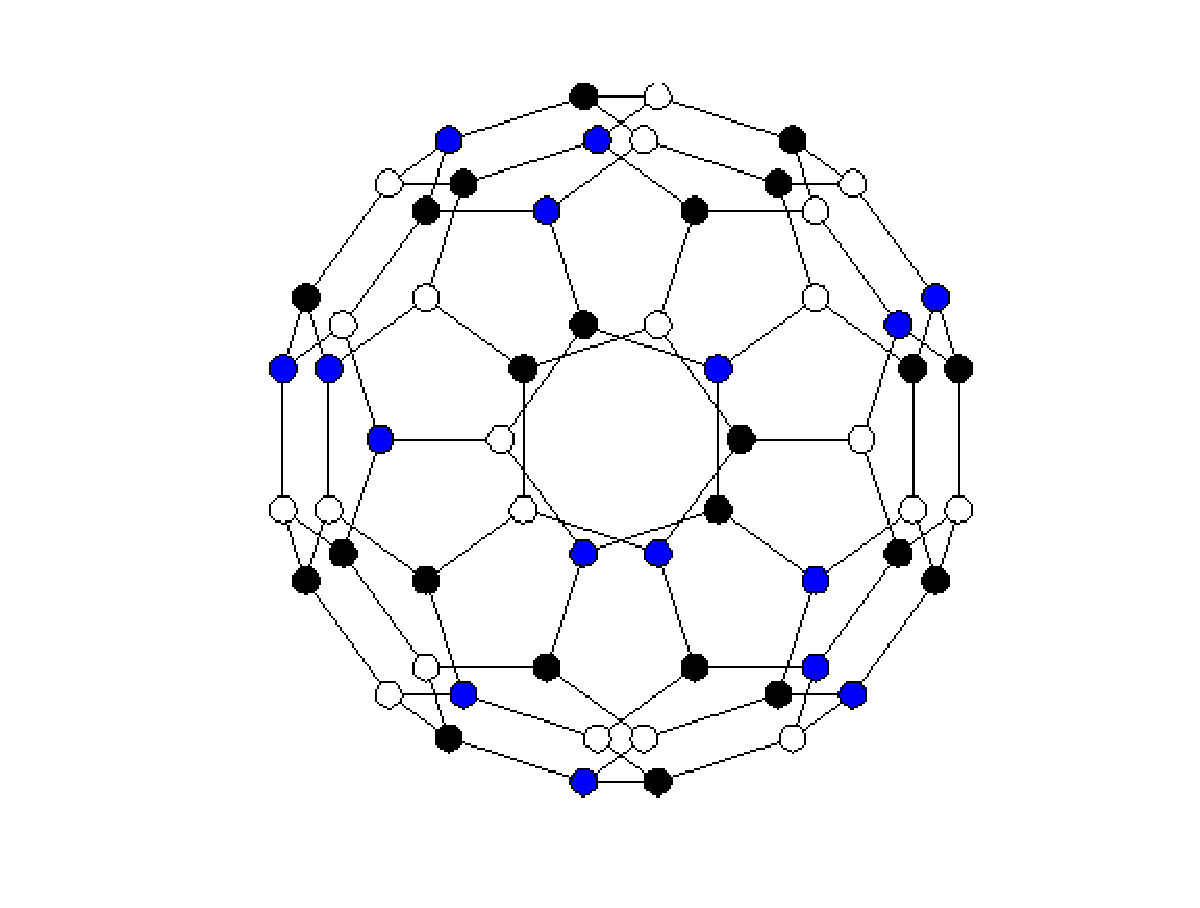
\includegraphics[scale=0.5]{figs/bucky}
  \end{center}
  \caption{An optimal coloring of the Bucky ball.}
  \label{fig:bucky}
\end{figure}
The \verb|cdraw| command draws a graph with a given coloring. Note
that the coloring need not be a proper coloring. Here is an example:
\begin{verbatim}
>> grid(g,5,5)
>> c = split(g);
>> clf; cdraw(g,c)
\end{verbatim}
The result is in Figure~\ref{fig:split-grid}.
\begin{figure}[ht]
  \begin{center}
    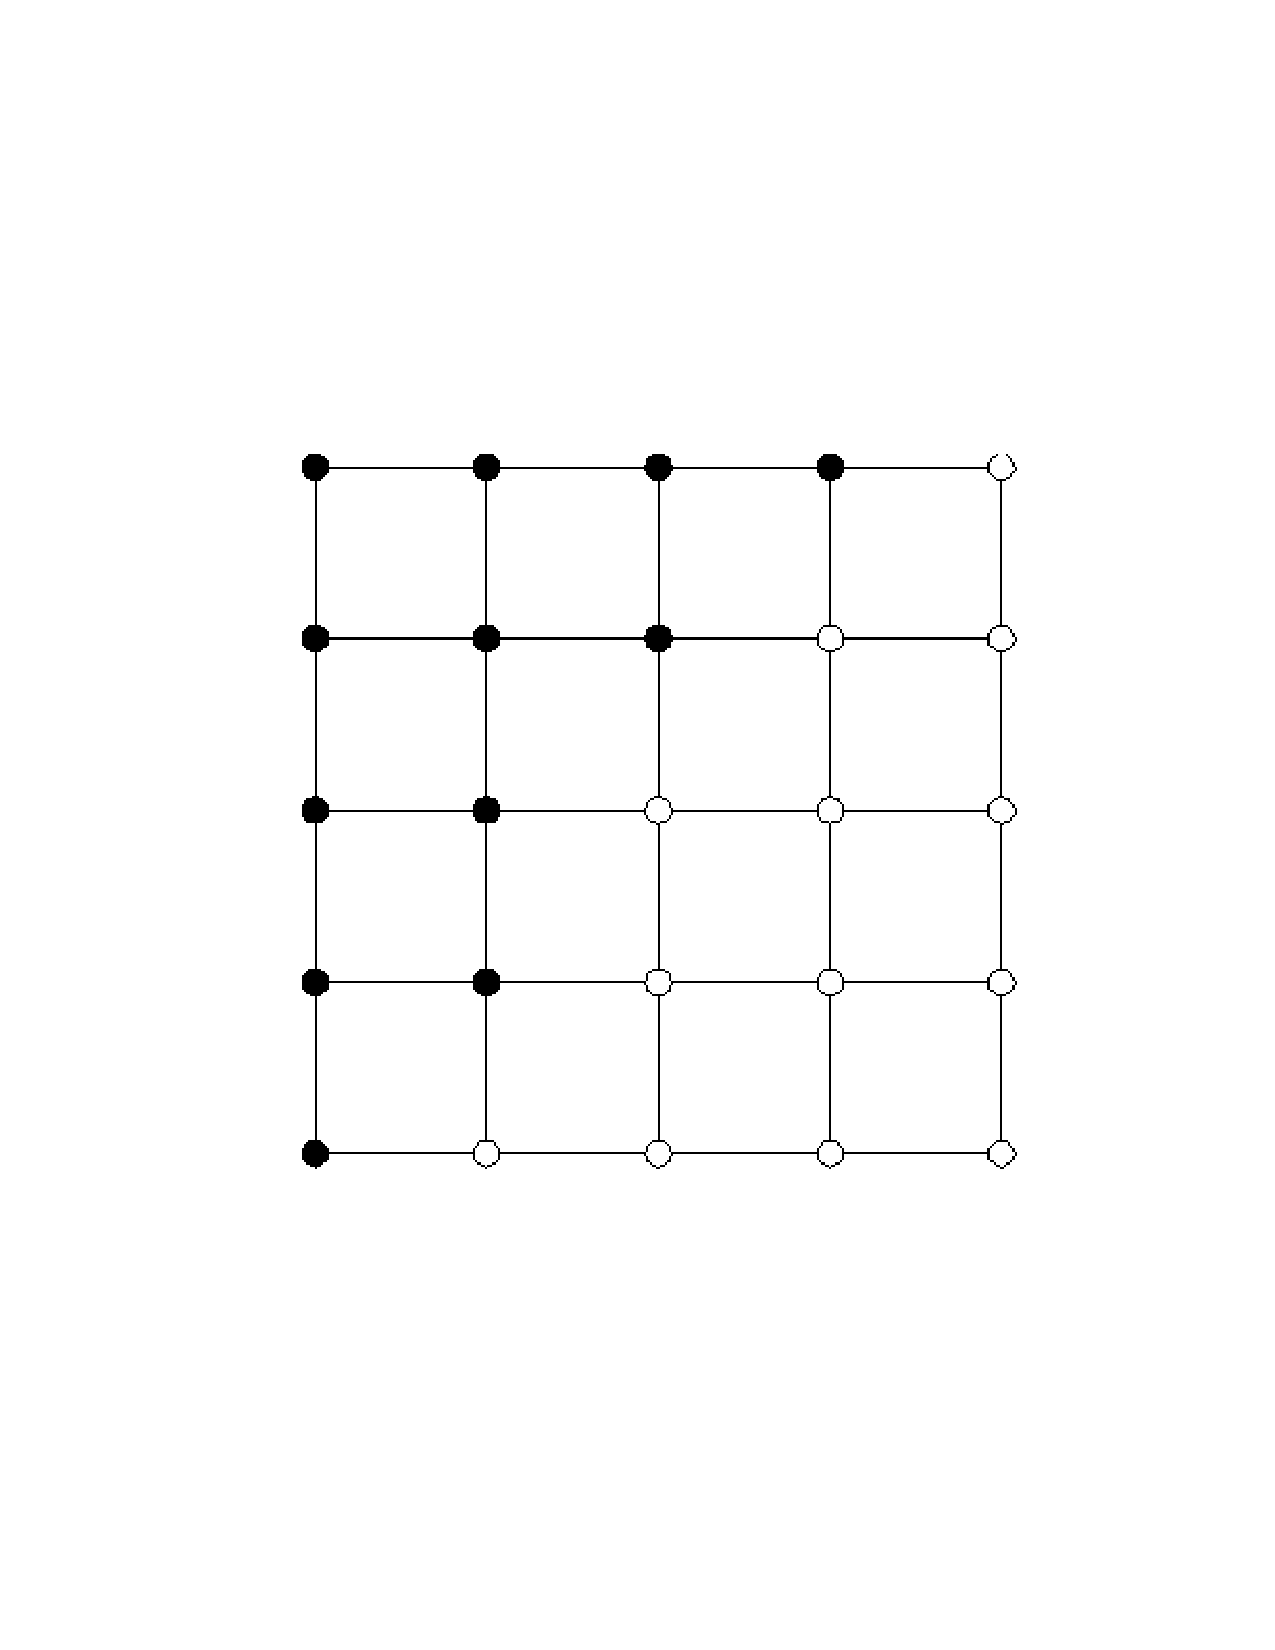
\includegraphics[scale=0.5]{figs/split-grid}
  \end{center}
  \caption{A $5\times5$ grid partitioned 
    into two sets of vertices by \texttt{split}.}
  \label{fig:split-grid}
\end{figure}

\matgraph\ can find the chromatic polynomial of small graphs.
\begin{verbatim}
>> cube(g,3)
>> chromatic_poly(g)
ans =
     1   -12    66  -214   441  -572   423  -133     0
\end{verbatim}
This tells us that
$$
\chi(Q_3;x) = x^8 -12 x^7 + 66 x^6 - 215 x^5 + 441 x^4 -572 x^3 +
423 x^2 -133 x .
$$

If a graph has a two-coloring (i.e., if the graph is bipartite) then
we can use \verb|bipartition| to find the two color classes.
\begin{verbatim}
>> cycle(g,8)
>> bipartition(g)
{ {1,3,5,7} {2,4,6,8} }
\end{verbatim}
Given a partition of a graph into two sets, we can find a maximum
matching between those sets with \verb|bipmatch|.
\begin{verbatim}
>> random_bipartite(g,6,6,.5)
>> bipartition(g)
{ {1,2,3,4,5,6} {7,8,9,10,11,12} }
>> bipmatch(g,ans)
ans =
     1     7
     2     8
     3     9
     4    11
     5    10
     6    12
\end{verbatim}


\section{Sparse Graphs}
Graphs in \matgraph\ are housed in symmetric matrices. \matlab\ can
hold matrices either as \emph{full} or \emph{sparse} arrays. The
amount of memory used by a full array is proportional to the number of
entries in the matrix, while the memory used by a sparse array is
proportional to the number of nonzero entries in the matrix. 

Graphs in \matgraph\ are held, behind the scenes, in either full or
sparse matrices. To find out which, use the functions \verb|isfull| or
\verb|issparse|. Alternatively, simply typing the graph variable's
name reveals its storage type.
\begin{verbatim}
>> petersen(g)
>> g
Graph with 10 vertices and 15 edges (full)
\end{verbatim}
For large graphs with relatively few edges, sparse storage is
preferable; indeed, full storage may not be feasible because the
computer might not have enough RAM to hold the matrix. To convert a
graph to sparse storage, simply type \verb|sparse(g)|. 
\begin{verbatim}
>> sparse(g)
>> cycle(g,1000)
>> g
Graph with 1000 vertices and 1000 edges (sparse)
\end{verbatim}
When declaring a new graph variable, one may specify the number of
vertices in the constructor: \verb|h = graph(n)|. If \verb|n| is large,
then sparse storage is used. 
\begin{verbatim}
>> k = graph(10000)
Graph with 10000 vertices and 0 edges (sparse)
\end{verbatim}
How large is ``large''? This is controlled by the function
\verb|set_large|. 
 

\section{Input and Output}

\subsection{Saving graphs to disk with \texttt{save} and \texttt{load}}
The usual mechanisms for saving variables to disk do not work for
\verb|graph| variables in \matgraph. Were you to attempt to save a
\verb|graph| variable, or the entire \matlab\ workspace, the graphs
you have created will be lost when you try to load them back in. This
is one of the prices we pay for creating a fast call-by-reference
system. 

Instead, \matgraph\ provides its own \verb|save| and \verb|load|
commands. \verb|save(g,filename)| saves the graph \verb|g| to a file
in the current directory on your hard drive. A subsequent call to
\verb|load(g,filename)| overwrites the graph \verb|g| with the graph
saved in the file. Here is an example:
\begin{verbatim}
>> g = graph
Graph system initialized. Number of slots = 500.
Graph with 0 vertices and 0 edges (full)
>> petersen(g)
>> save(g,'pete')
>> free(g)
>> g
Invalid graph object (index 1)
>> clear g
>> g = graph
Graph with 0 vertices and 0 edges (full)
>> g
Graph with 0 vertices and 0 edges (full)
>> load(g,'pete')
>> g
Graph with 10 vertices and 15 edges (full) 
\end{verbatim}


\subsection{SGF: Simple Graph Format}
\label{sect:sgf}
The \matgraph\ function \verb|sgf| is a mechanism to convert
\verb|graph| objects to and from a two-column matrix format called
Simple Graph Format. For a graph with $n$ vertices and $m$ edges, the
Simple Graph Format matrix has either $m+1$ or $n+m+1$ rows. The first
row of the matrix gives the number of vertices and the number of edges
in the graph. The following $m$ rows specify the edges of the
graph. Optionally, an additional $n$ rows specify the
$x,y$-coordinates of the embedding of the graph. Here is an example.
\begin{verbatim}
>> complete(g,4)
>> sgf(g)
ans =
     4     6
     1     2
     1     3
     2     3
     1     4
     2     4
     3     4
>> distxy(g)
Optimization terminated: relative function value
 changing by less than OPTIONS.TolFun.
Embedding score = 0.34315
Elapsed time is 0.079532 seconds.
ans =
    0.3431
>> sgf(g)
ans =
    4.0000    6.0000
    1.0000    2.0000
    1.0000    3.0000
    2.0000    3.0000
    1.0000    4.0000
    2.0000    4.0000
    3.0000    4.0000
    1.3651    1.3939
    1.2374    2.5943
    0.7011    1.9303
    1.9014    2.0580
\end{verbatim}

Not only can \verb|sgf| be used to create a Simple Graph Format matrix
from a graph, it can also be used to specify a graph. For example,
here we create the SGF matrix for the graph $K_{1,5}$ and an embedding
using \matlab\ commands, and then build a graph based on that matrix.
\begin{verbatim}
>> edges = [ ones(5,1), [2:6]' ]
edges =
     1     2
     1     3
     1     4
     1     5
     1     6
>> xy = [ 0 0 ; -2 1 ; -1 1 ; 0 1 ; 1 1 ; 2 1 ];
>> S = [ 6 5 ; edges ; xy ]
S =
     6     5
     1     2
     1     3
     1     4
     1     5
     1     6
     0     0
    -2     1
    -1     1
     0     1
     1     1
     2     1
>> sgf(g,S)
>> clf;draw(g)
\end{verbatim}
The result is show in Figure~\ref{fig:star}.
\begin{figure}[ht]
  \begin{center}
    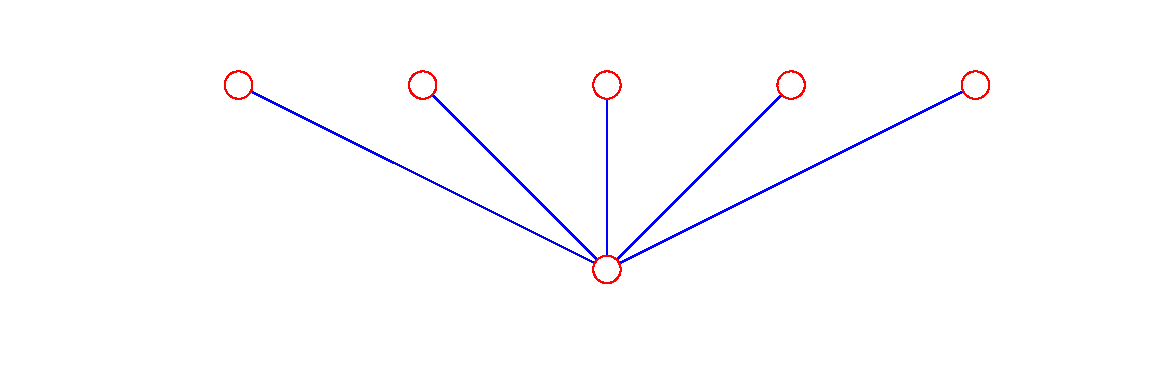
\includegraphics[scale=0.5]{figs/star}
  \end{center}
  \caption{A star graph created using a Simple Graph Format matrix.}
  \label{fig:star}
\end{figure}

The Simple Graph Format is useful for working with other computing
environments. You may have, say, a C++ program that you use to create
graphs. You can have that program write the graph to disk in simple
graph format. Then, using the usual \matlab\ \verb|load| command, the
two-column matrix can be read from disk and converted into a graph.



\subsection{A C++ graph parser} 
Inside the main \matgraph\ directory, you can find a subdirectory
named \verb|tools| that contains a further subdirectory named
\verb|graph_parser|. This directory contains a C++ program to build a
command-line tool that reads textual graph data from the standard
input and writes its output to a file named
\verb|parsed_graph.m|. This can then be converted into a graph in
\matgraph\ by giving the command \verb|parsed_graph(g)|. Here are the
steps you need to take to make this work.

\subsubsection*{Compile the program}
We assume basic knowledge of the Unix shell (Linux, Mac OS X, Cygwin
on Windows, etc.) and that your computer has a C++ compiler installed.
(This has been tested using the GNU compiler \verb|g++|.) 

To build the program, simply change directory to the
\verb|graph_parser| directory and type \verb|make|:
\begin{verbatim}
$ cd /home/username/matgraph/tools/graph_parser/
$ make
g++ -ansi -O   -c -o main.o main.cc
g++ -ansi -O   -c -o LineParser.o LineParser.cc
g++ main.o LineParser.o -o graph_parser
$
\end{verbatim}
The program \verb|graph_parser| is created. This can be moved to any
convenient location.

\subsubsection*{Graph data file}
The \verb|graph_parser| program reads a specific type of data
file. Vertices are named as character strings (henceforth, ``words'')
such as \verb|head-node| or \verb|city| or \verb|123|. No white space
may appear in the name of a vertex and vertex names are case sensitive
(the word \verb|hello| is not the same as \verb|Hello|).

A typical line in the data file contains the name of exactly two
words; such a line indicates that there is an edge between the
named vertices. If there are more than two words on a line, only the
first two words are processed; the rest of the line is ignored.

In order to accommodate isolated vertices, a line in the data file may
contain just a single word. This tells \verb|graph_parser| that the
given word is the name of a vertex. If this word has not been
previously encountered (e.g., on a previous line as part of an edge),
then this names a new vertex in the graph. 

If a line begins with the same word twice, the second instance of the
word is ignored and this line is treated as if it contained only one
word.

Finally, if a line is blank or if a line begins with the sharp
character \verb|#|, then the line is ignored (this is useful for
annotating the data file). 

A typical input file (named \verb|test|) is included in the
\verb|graph_parser| directory; we show the contents of that file here:
\begin{verbatim}
one two
one             three
four
five two
two six      and the rest of this line is ignored
seven
eight nine
nine two
one one   <-- a loop is not created
two nine

eight seven
eight one  fifty
four six
seven six
four five
   three five
# this line should be skipped
nine seven
\end{verbatim}


\subsubsection*{Convert the data file into a \texttt{.m} file}

Once the data file is prepared, we use \verb|graph_parser| to convert
the data file into a \verb|.m| file that can be run in \matlab. In the
shell, give the following command:
\begin{verbatim}
./graph_parser < filename
\end{verbatim}
where \verb|filename| is the name of the file containing the graph
data. The result of running the program \verb|graph_parser| is the
creation of a file named \verb|parsed_graph.m| in the same directory
in which \verb|graph_parser| was run. You need to have write
permission for that directory or \verb|graph_parser| will complain:
\begin{verbatim}
Unable to open file parsed_graph.m for output
\end{verbatim}

The file \verb|parsed_graph.m| can be moved to any convenient
location. You should not change the name of this file because it is a
\matlab\ function. If you wish to process two (or more) graph files,
run \verb|graph_parser| on the first data file and then read the graph
into \matlab\ (explained next) before processing subsequent data
files.


\subsubsection*{Run the \texttt{.m} file in \matlab}

The final step is to execute the function \verb|parsed_graph| inside
\matlab.
\begin{verbatim}
>> parsed_graph(g)
>> g
Graph with 9 vertices and 13 edges (full)
>> distxy(g)
Optimization terminated: relative function value
 changing by less than OPTIONS.TolFun.
Embedding score = 2.5448
Elapsed time is 0.210241 seconds.
ans =
    2.5448
>> ldraw(g)
\end{verbatim}
The graph defined textually in \verb|test| is now saved as
\verb|graph| object in \matgraph\ and can be handled like any other
such graph. The drawing of this graph is shown in
Figure~\ref{fig:parsed}.
\begin{figure}[ht]
  \begin{center}
    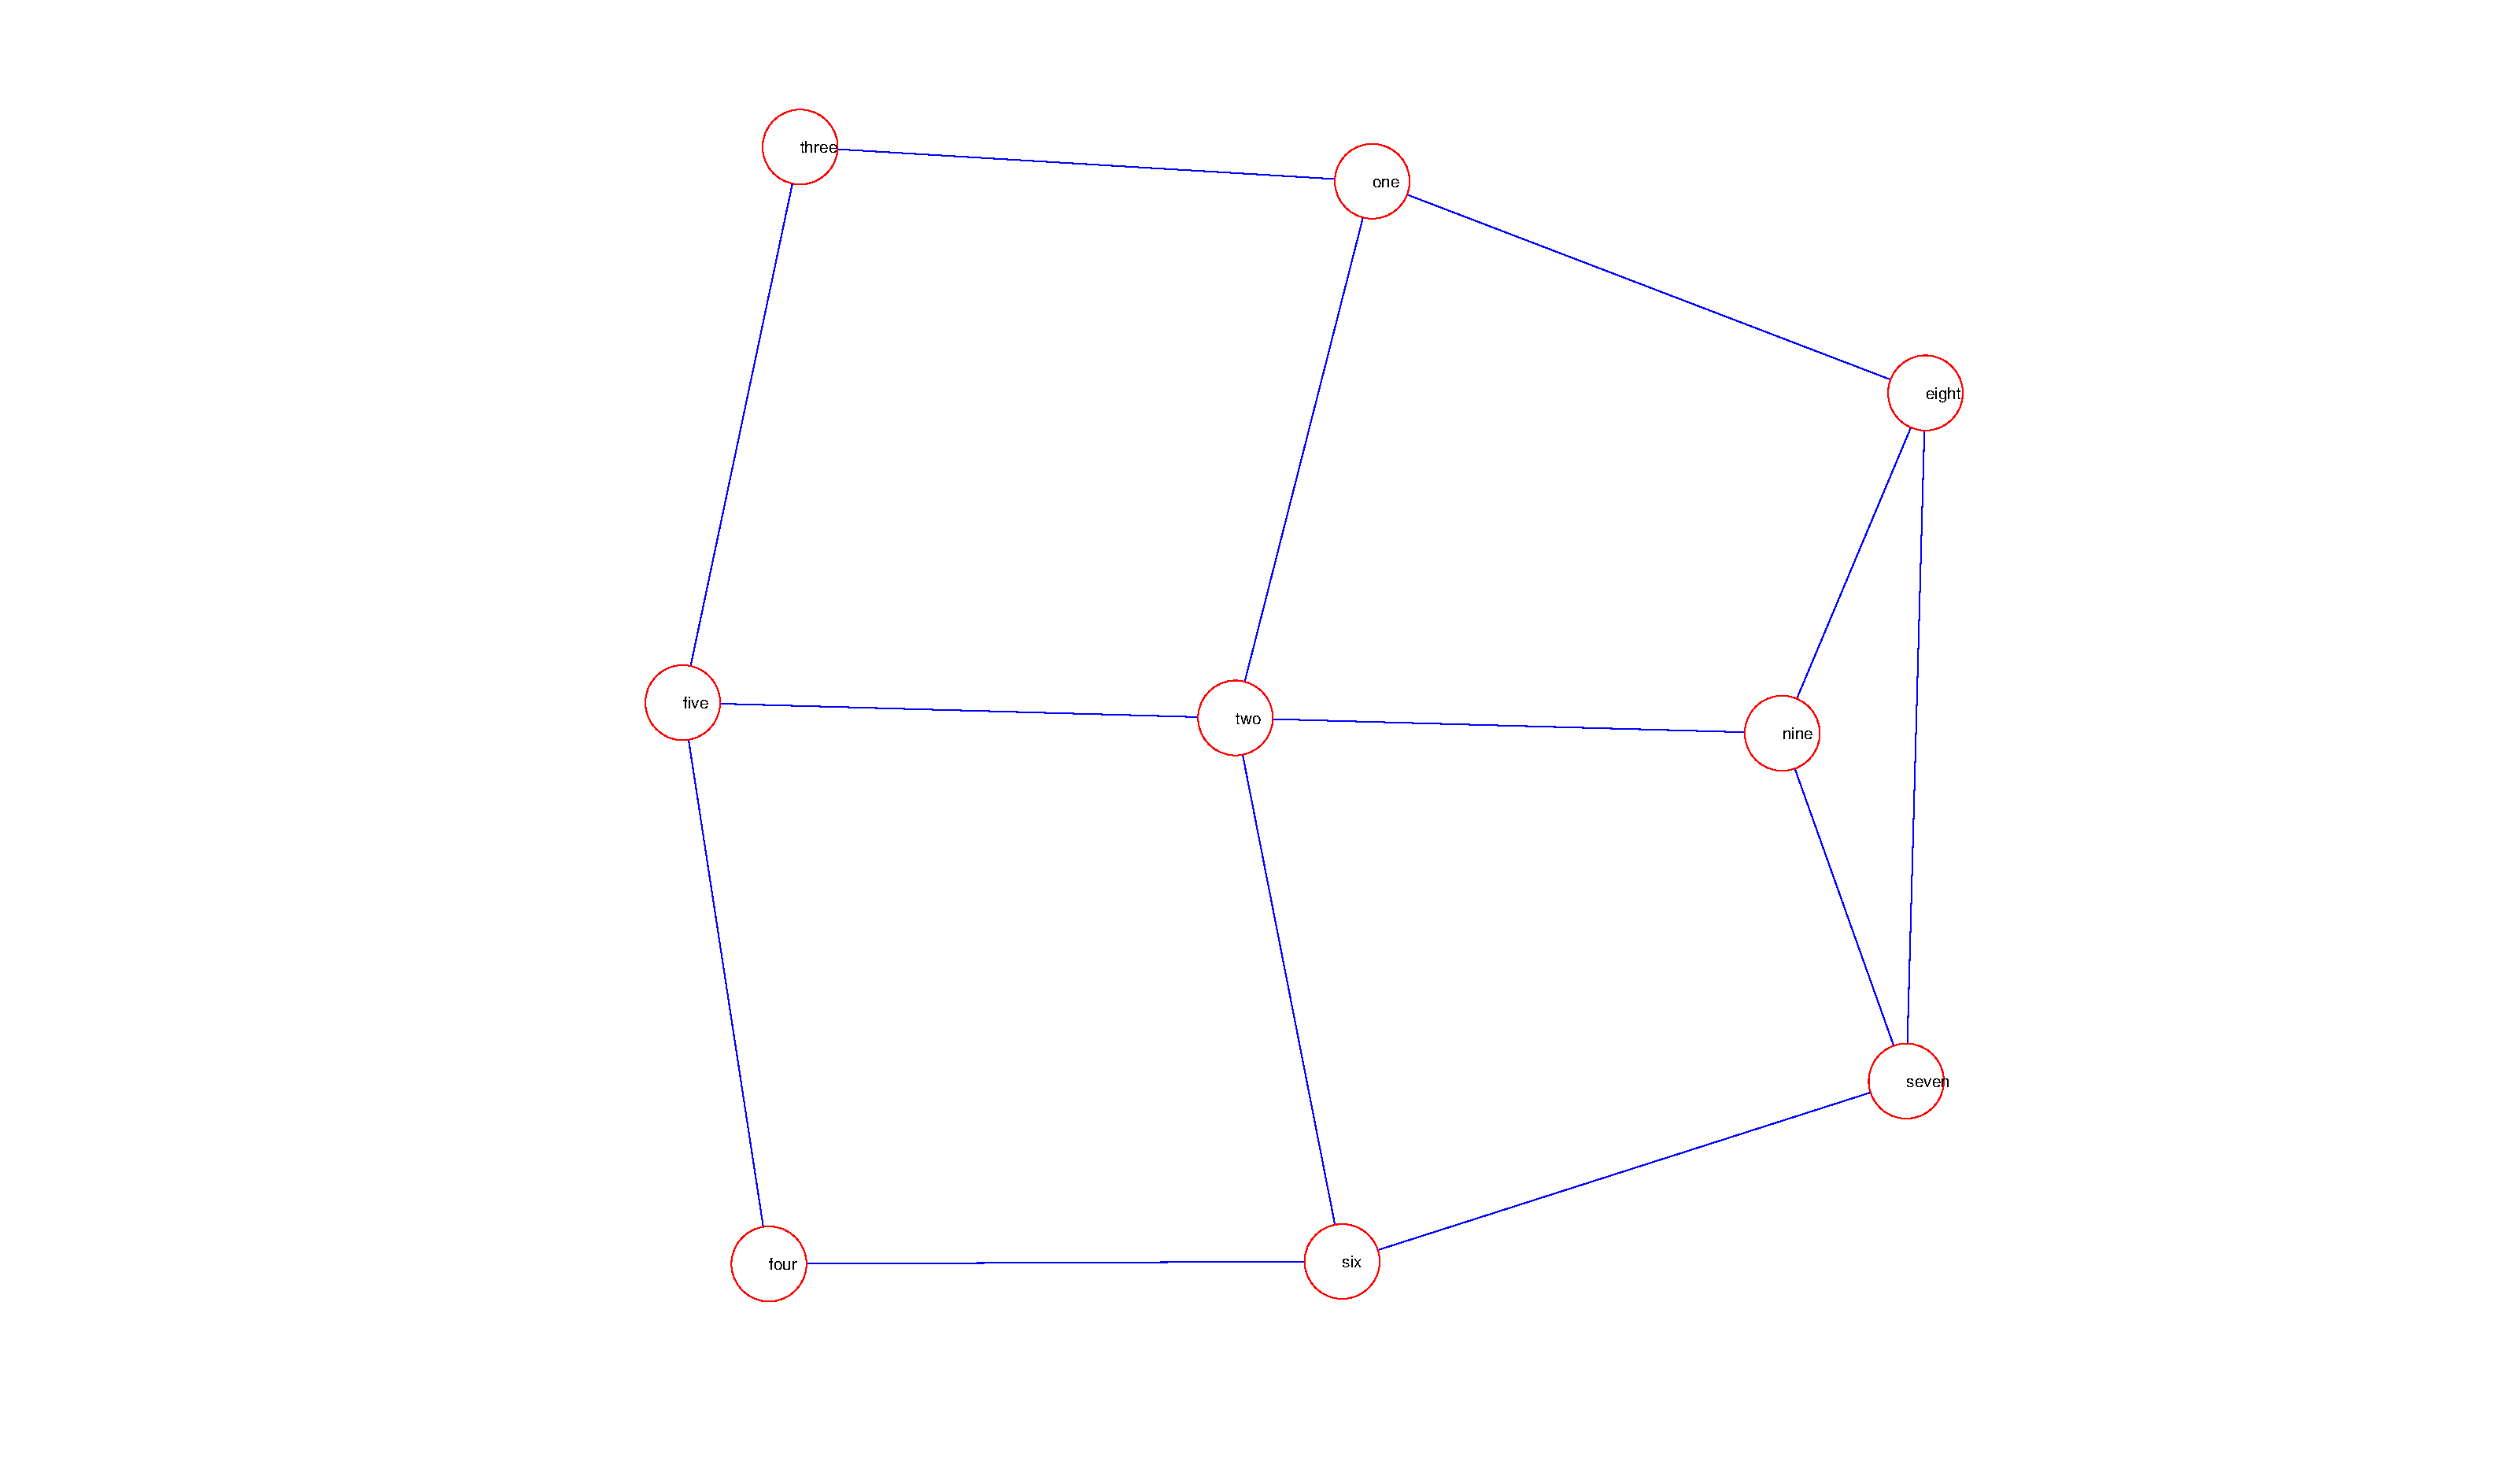
\includegraphics[width=\textwidth]{figs/parsed}
  \end{center}
  \caption{A drawing of a graph read into \matgraph\ via the
    \texttt{graph\_parser} program.}
  \label{fig:parsed}
\end{figure}


\subsection {Connecting with other programs}

It is possible to create \matlab\ programs to write graphs to files in
other formats. Included with \matgraph\ are ways to do this for
Graphviz and OmniGraffle.

\subsubsection*{Saving graphs for Graphviz}

Graphviz is a graph visualization tool available from the website
\begin{verbatim}
http://www.graphviz.org/
\end{verbatim}
One of the Graphviz tools is named \verb|dot|, and \matgraph\ includes
a function also named \verb|dot| to convert \verb|graph| objects into
a format that can be read by Graphviz's \verb|dot|. The \matgraph\
command has the form \verb|dot(g,'filename.dot')|. This writes a file
to the computer's disk that can then be used by Graphviz. Here is an
example of how to do this:
\begin{verbatim}
>> cube(g,4)
>> dot(g,'four-cube.dot')
Wrote "four-cube.dot"
\end{verbatim}
The file \verb|four-cube.dot| is now read into a Graphviz tool to
produce attractive drawings such as the one shown in
Figure~\ref{fig:four-cube}.
\begin{figure}[ht]
  \begin{center}
    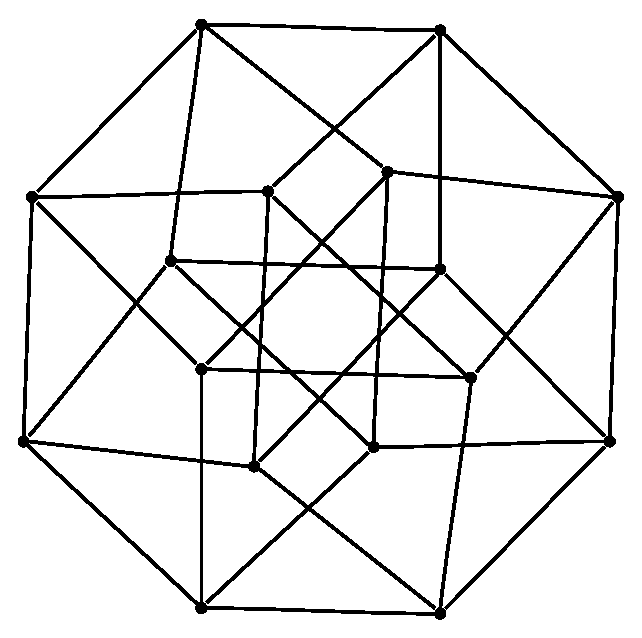
\includegraphics[scale=0.5]{figs/four-cube}
  \end{center}
  \caption{A picture of $Q_4$ produced by exporting a graph from
    \matgraph\ and then laid out using GraphViz.}
  \label{fig:four-cube}
\end{figure}
See the Graphviz website for more information.


\subsubsection*{Saving graphs for OmniGraffle}

OmniGraffle is a graph drawing program for Macintosh available from
this website:
\begin{verbatim}
http://www.omnigroup.com/
\end{verbatim}
\matgraph\ can save graphs in a format that can be read by
OmniGraffle. The \matgraph\ command \verb|graffle(g,'filename.graffle')| writes
the graph to disk. Double clicking the created file launches
OmniGraffle. Here's an example:
\begin{verbatim}
>> cube(g,3)
>> graffle(g,'cube.graffle')
\end{verbatim}
Using OmniGraffle's layout tool, we can produce a nice embedding of
the graph as shown in Figure~\ref{fig:graffle}.
\begin{figure}[ht]
  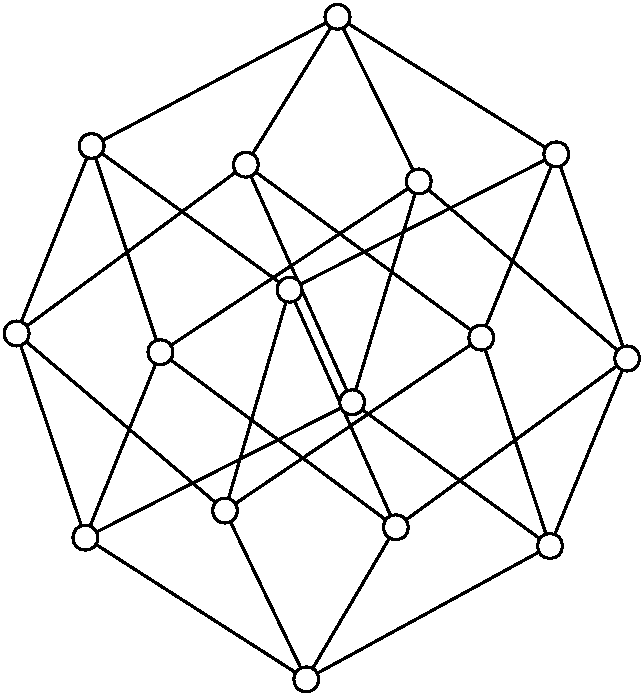
\includegraphics[scale=0.5]{figs/graffle}
  \caption{A picture of $Q_4$ produced by exporting a graph from
    \matgraph\ and then laid out using OmniGraffle.}
  \label{fig:graffle}
\end{figure}

To a limited extent, it is possible to convert graphs prepared in
OmniGraffle for import into \matgraph. Inside the
\verb|matgraph/tools| directory resides a program named
\verb|graffle2sgf.py|. This is a Python language program so, in order
to run it you must have Python installed on your computer.  This
program takes as input a graph saved by OmniGraffle and returns as
output a matrix specifying the graph in Simple Graph Format (see
\S\ref{sect:sgf}).

Suppose you have created a graph using OmniGraffle and saved it on
your hard disk in a 
file called \verb|mygraph.graffle|. Issue the following command in the
Unix shell:
\begin{verbatim}
./graffle2sgf.py < mygraph.graffle > mygraph
\end{verbatim}
This reads the graph saved by OmniGraffle and writes the relevant data
into the file \verb|mygraph|.

Now, inside \matlab, do the following:
\begin{verbatim}
>> load mygraph
>> sgf(g,mygraph)
>> g
Graph with 5 vertices and 6 edges (full)
\end{verbatim}
The \matlab\ command \verb|load mygraph| reads the file \verb|mygraph|
and saves the matrix contained therein into a variable that is also
named \verb|mygraph|. The command \verb|sgf(g,mygraph)| overwrites
\verb|g| with the graph specified by the SGF matrix \verb|mygraph|. 

The \verb|graffle2sgf.py| tool is not completely reliable. It works
well on diagrams that contain only nodes and edges. If there are other
extraneous lines or text in the diagram (which an OmniGraffle diagram
certainly may have), then the program can get confused and give poor
performance. Readers are invited to submit a better version.

\end{document}

%%% Local Variables: 
%%% mode: latex
%%% TeX-master: t
%%% End: 
